\documentclass[11pt]{article}

\usepackage[a4paper,margin=25mm]{geometry}
\usepackage{amsmath,amssymb,bm,booktabs,graphicx,hyperref}
\hypersetup{hidelinks}
\graphicspath{{figures/review/}}
\setlength{\parindent}{0pt}
\setlength{\parskip}{6pt}

\title{Supporting Information for ``A generalized gamma kernel-machine promotion-time cure model''}
\author{Gabriel de Jesus Pereira \and Vera L. D. Tomazella \and Pedro R. D. Marinho \and Marcelo Rodrigo Portela Ferreira \and Agatha S. Rodrigues}
\date{}

\begin{document}
\maketitle

\section{Likelihood construction and conditional blocks}\label{sec:supp-likelihood}

\subsection{Observed and complete-data likelihoods}

The observed time is $Y_i=\min(T_i,C_i)$, its realized value
is $t_i$, and $\delta_i=I(T_i\leq C_i)$. The observed data
are $\mathcal D_{\mathrm{obs}}=\{(t_i,\delta_i,\bm{x}_i)\}_{i=1}^{n}$,
and the complete data augment these observations with the
latent counts $N_i$. The full predictor is $\eta_i=\beta_0+\bm K_i^{\mathsf T}\bm\alpha$,
with $\theta_i=\exp(\eta_i)$; the symbol $f$ is reserved for
the RKHS component in $\eta(\bm{x})=\beta_0+f(\bm{x})$.
Throughout, $K(\cdot,\cdot)$ is assumed to be a symmetric
positive-semidefinite kernel, and $\bm K$ denotes the corresponding
Gram matrix with entries $K(\bm x_i,\bm x_j)$. By the representer
theorem, $f(\bm x)=\sum_{j=1}^{n}\alpha_jK(\bm x,\bm x_j)$ and
$\|f\|_{\mathcal H_K}^2=\bm\alpha^{\mathsf T}\bm K\bm\alpha$.
Write $F_i=F_{GG}(t_i;a,d,p)$, $S_i=S_{GG}(t_i;a,d,p)=1-F_i$,
and $f_{GG,i}=f_{GG}(t_i;a,d,p)$. The parameter vectors are
$\bm\Theta_{\mathrm P}=(\beta_0,\bm\alpha,a,d,p)$ and
$\bm\Theta_{\mathrm{NB}}=(\beta_0,\bm\alpha,a,d,p,\phi)$.

Let $\pi_k(\bm{x}_i)=P(N_i=k\mid\bm{x}_i)$ and
$A_i(u)=\sum_{k\geq0}\pi_k(\bm{x}_i)u^k$. Conditional on
$N_i=n_i\geq1$, the event time is the minimum of $n_i$
independent activation times. Hence
\begin{equation}
\begin{aligned}
P(T_i>t_i\mid N_i=n_i,\bm{x}_i)&=S_i^{n_i},\\
f_{T_i\mid N_i,\bm{x}_i}(t_i\mid n_i,\bm{x}_i)
&=-\frac{\mathrm d}{\mathrm dt_i}S_i^{n_i}
=n_i f_{GG,i}S_i^{n_i-1}.
\end{aligned}
\label{eq:supp-conditional-event-time}
\end{equation}
When $N_i=0$, $T_i=\infty$, so the conditional survival is
one and an observed event is impossible. Under independent,
noninformative censoring, the censoring contribution contains
no parameters of interest and is omitted from the likelihood
below. Combining event and censoring contributions gives
\begin{equation}
\begin{aligned}
L_{c,i}(\bm\Theta;n_i)
&=\pi_{n_i}(\bm{x}_i)
\{n_i f_{GG,i}S_i^{n_i-1}\}^{\delta_i}
\{S_i^{n_i}\}^{1-\delta_i}\\
&=\pi_{n_i}(\bm{x}_i)n_i^{\delta_i}
f_{GG,i}^{\delta_i}S_i^{n_i-\delta_i},
\qquad n_i\geq\delta_i.
\end{aligned}
\label{eq:supp-complete-contribution}
\end{equation}
For a censored observation, $n_i^{0}$ is interpreted as one,
including when $n_i=0$. The complete-data likelihood is the
product of these contributions, and its logarithm is
\begin{equation}
\ell_c(\bm\Theta;\mathcal D_{\mathrm{comp}})
=\sum_{i=1}^{n}\Bigl[
\log\pi_{N_i}(\bm{x}_i)+\delta_i\log N_i
+\delta_i\log f_{GG,i}+(N_i-\delta_i)\log S_i
\Bigr].
\label{eq:supp-generic-complete-loglikelihood}
\end{equation}
The term $\delta_i\log N_i$ is evaluated only for observed
events, for which $N_i\geq1$; its contribution is zero for
censored observations.

Summing Equation~\eqref{eq:supp-complete-contribution} over
the latent count recovers the observed-data contribution:
\begin{equation}
\begin{aligned}
L_i(\bm\Theta)
&=f_{GG,i}^{\delta_i}
\sum_{k\geq\delta_i}\pi_k(\bm{x}_i)k^{\delta_i}S_i^{k-\delta_i}\\
&=\{f_{GG,i}A_i'(S_i)\}^{\delta_i}
\{A_i(S_i)\}^{1-\delta_i}.
\end{aligned}
\label{eq:supp-observed-contribution}
\end{equation}
Thus the population survival and density are $A_i\{S_{GG}(t)\}$ and $f_{GG}(t)A_i'\{S_{GG}(t)\}$, respectively, and the cure fraction is $A_i(0)=\pi_0(\bm{x}_i)$.

\subsection{Poisson and negative-binomial count laws}

For the Poisson specification, $N_i\mid\bm{x}_i\sim\operatorname{Poisson}(\theta_i)$, so
\begin{equation}
\pi_{n_i}(\bm{x}_i)
=\frac{e^{-\theta_i}\theta_i^{n_i}}{\Gamma(n_i+1)},
\qquad n_i=0,1,\ldots.
\label{eq:supp-poisson-count-pmf}
\end{equation}
Substituting this mass function into Equation~\eqref{eq:supp-generic-complete-loglikelihood} yields
\begin{equation}
\begin{aligned}
\ell_{c,\mathrm P}
={}&\sum_{i=1}^{n}\Bigl[
N_i\eta_i-\theta_i-\log\Gamma(N_i+1)+\delta_i\log N_i\\
&\hspace{30mm}+\delta_i\log f_{GG,i}+(N_i-\delta_i)\log S_i
\Bigr].
\end{aligned}
\label{eq:supp-poisson-complete-loglikelihood}
\end{equation}
The Poisson generating function is $A_i(u)=\exp\{\theta_i(u-1)\}$, with $A_i'(u)=\theta_i A_i(u)$. Consequently, the censored and event contributions in Equation~\eqref{eq:supp-observed-contribution} are $\exp(-\theta_iF_i)$ and $\theta_i f_{GG,i}\exp(-\theta_iF_i)$. The observed penalized log-likelihood is therefore
\begin{equation}
\ell_{\mathrm P}^{\mathrm{pen}}(\bm\Theta_{\mathrm P})
=\sum_{i=1}^{n}\bigl[\delta_i\{\eta_i+\log f_{GG,i}\}-\theta_iF_i\bigr]
-\frac{\lambda}{2}\bm\alpha^{\mathsf T}\bm K\bm\alpha.
\label{eq:supp-poisson-observed-loglikelihood}
\end{equation}

For the negative-binomial specification, the mean is $\theta_i$ and the dispersion is $\phi>0$, with variance $\theta_i(1+\phi\theta_i)$. Its mass function is
\begin{equation}
\pi_{n_i}(\bm{x}_i)
=\frac{\Gamma(n_i+\phi^{-1})}
{\Gamma(\phi^{-1})\Gamma(n_i+1)}
\frac{(\phi\theta_i)^{n_i}}
{(1+\phi\theta_i)^{n_i+\phi^{-1}}},
\qquad n_i=0,1,\ldots.
\label{eq:supp-nb-count-pmf}
\end{equation}
Its substitution into the generic complete-data log-likelihood gives
\begin{equation}
\begin{aligned}
\ell_{c,\mathrm{NB}}
={}&\sum_{i=1}^{n}\Bigl[
\log\Gamma(N_i+\phi^{-1})-\log\Gamma(\phi^{-1})
-\log\Gamma(N_i+1)\\
&\quad+N_i(\log\phi+\eta_i)
-(N_i+\phi^{-1})\log(1+\phi\theta_i)\\
&\quad+\delta_i\log N_i+\delta_i\log f_{GG,i}
+(N_i-\delta_i)\log S_i
\Bigr].
\end{aligned}
\label{eq:supp-nb-complete-loglikelihood}
\end{equation}
The generating function and its first derivative are
\begin{equation}
\begin{aligned}
A_i(u)&=\{1+\phi\theta_i(1-u)\}^{-1/\phi},\\
A_i'(u)&=\theta_i\{1+\phi\theta_i(1-u)\}^{-1/\phi-1}.
\end{aligned}
\label{eq:supp-nb-generating-function}
\end{equation}
Writing $D_i=1+\phi\theta_iF_i$, the corresponding censored and event contributions are $D_i^{-1/\phi}$ and $\theta_i f_{GG,i}D_i^{-1/\phi-1}$. Hence
\begin{equation}
\ell_{\mathrm{NB}}^{\mathrm{pen}}(\bm\Theta_{\mathrm{NB}})
=\sum_{i=1}^{n}\Bigl[
\delta_i\{\eta_i+\log f_{GG,i}\}
-(\phi^{-1}+\delta_i)\log D_i
\Bigr]
-\frac{\lambda}{2}\bm\alpha^{\mathsf T}\bm K\bm\alpha.
\label{eq:supp-nb-observed-loglikelihood}
\end{equation}

\subsection{Conditional latent counts}

At iteration $r$, all conditional expectations are taken under the current estimate $\bm\Theta^{(r)}$. To derive them, first suppress the iteration index and let $A_i^{(j)}$ denote the $j$th derivative of the generating function, with $A_i^{(0)}=A_i$. Bayes' rule and Equation~\eqref{eq:supp-observed-contribution} imply
\begin{equation}
P(N_i=k\mid t_i,\delta_i,\bm{x}_i;\bm\Theta)
=\frac{\pi_k(\bm{x}_i)k^{\delta_i}S_i^{k-\delta_i}}
{A_i^{(\delta_i)}(S_i)},
\qquad k\geq\delta_i.
\label{eq:supp-count-posterior}
\end{equation}
For a censored observation, the conditional mean is $S_iA_i'(S_i)/A_i(S_i)$. For an observed event, the identity $k^2=k(k-1)+k$ gives the conditional mean $1+S_iA_i''(S_i)/A_i'(S_i)$. The two cases combine as
\begin{equation}
\mathbb E(N_i\mid t_i,\delta_i,\bm{x}_i;\bm\Theta)
=\delta_i+S_i
\frac{A_i^{(\delta_i+1)}(S_i)}
{A_i^{(\delta_i)}(S_i)}.
\label{eq:supp-generic-estep}
\end{equation}

For Poisson counts, $A_i'/A_i=A_i''/A_i'=\theta_i$; equivalently, the posterior distribution of $N_i-\delta_i$ is Poisson with mean $\theta_iS_i$. Restoring the iteration index yields
\begin{equation}
\widehat N_{i,\mathrm P}^{(r)}
=\mathbb E_{\bm\Theta_{\mathrm P}^{(r)}}
(N_i\mid t_i,\delta_i,\bm{x}_i)
=\delta_i+\theta_i^{(r)}S_{GG}^{(r)}(t_i).
\label{eq:supp-poisson-estep}
\end{equation}
For negative-binomial counts, Equation~\eqref{eq:supp-nb-generating-function} gives
\begin{equation}
\frac{A_i'(S_i)}{A_i(S_i)}=\frac{\theta_i}{D_i},
\qquad
\frac{A_i''(S_i)}{A_i'(S_i)}
=\frac{(1+\phi)\theta_i}{D_i}.
\end{equation}
Substitution into Equation~\eqref{eq:supp-generic-estep} gives
\begin{equation}
\widehat N_{i,\mathrm{NB}}^{(r)}
=\delta_i+
\frac{(1+\phi^{(r)}\delta_i)\theta_i^{(r)}S_{GG}^{(r)}(t_i)}
{1+\phi^{(r)}\theta_i^{(r)}F_{GG}^{(r)}(t_i)}.
\label{eq:supp-nb-estep}
\end{equation}
These conditional counts are computed once per E-step and held fixed throughout the subsequent conditional maximizations.

\subsection{Conditional objectives and the dispersion update}

The penalized auxiliary function is
\begin{equation}
Q_\lambda(\bm\Theta\mid\bm\Theta^{(r)})
=\mathbb E_{\bm\Theta^{(r)}}
\{\ell_c(\bm\Theta;\mathcal D_{\mathrm{comp}})
\mid\mathcal D_{\mathrm{obs}}\}
-\frac{\lambda}{2}\bm\alpha^{\mathsf T}\bm K\bm\alpha.
\label{eq:supp-penalized-Q}
\end{equation}
In the Poisson case, the expectations of $-\log\Gamma(N_i+1)$ and $\delta_i\log N_i$ are constant with respect to the candidate parameters. They generally do not vanish, but they may be omitted from maximization. In the negative-binomial case, the terms involving $\log\Gamma(N_i+\phi^{-1})$, $\log\Gamma(\phi^{-1})$, and $N_i\log\phi$ are also constant with respect to the predictor and latency parameters when $\phi$ is fixed; they cannot be omitted when maximizing the expected complete-data criterion with respect to $\phi$.

Suppressing the iteration index on the fixed conditional counts, the predictor blocks follow directly from Equations~\eqref{eq:supp-poisson-complete-loglikelihood} and \eqref{eq:supp-nb-complete-loglikelihood}:
\begin{equation}
Q_{\eta,\mathrm P}
=\sum_{i=1}^{n}\{\widehat N_i\eta_i-\exp(\eta_i)\}
-\frac{\lambda}{2}\bm\alpha^{\mathsf T}\bm K\bm\alpha,
\label{eq:supp-poisson-predictor}
\end{equation}
and, for fixed $\phi$,
\begin{equation}
Q_{\eta,\mathrm{NB}}
=\sum_{i=1}^{n}\Bigl[
\widehat N_i\eta_i-(\widehat N_i+\phi^{-1})
\log\{1+\phi\exp(\eta_i)\}
\Bigr]
-\frac{\lambda}{2}\bm\alpha^{\mathsf T}\bm K\bm\alpha.
\label{eq:supp-nb-predictor}
\end{equation}
Both count laws share the latency block
\begin{equation}
Q_{GG}
=\sum_{i=1}^{n}\bigl[
\delta_i\log f_{GG,i}+(\widehat N_i-\delta_i)\log S_i
\bigr].
\label{eq:supp-latency-block}
\end{equation}
Thus the predictor and latency parameters can be updated separately after the E-step. For the negative-binomial model, direct maximization in $\phi$ would additionally require conditional expectations of functions such as $\log\Gamma(N_i+\phi^{-1})$. The ECME step instead maximizes the observed log-likelihood in $\phi$, after the predictor and latency updates:
\begin{equation}
\phi^{(r+1)}
=\underset{\phi>0}{\arg\max}\;
\ell_{\mathrm{NB}}^{\mathrm{pen}}
\bigl(\beta_0^{(r+1)},\bm\alpha^{(r+1)},
a^{(r+1)},d^{(r+1)},p^{(r+1)},\phi\bigr).
\label{eq:supp-ecme-dispersion}
\end{equation}
Because the RKHS penalty does not involve $\phi$, this is also the conditional maximization of the unpenalized observed log-likelihood. These are the objective functions and conditional expectations used in Algorithms 1 and 2 of the main article.

\section{Analytical scores and numerical parameterization}\label{sec:supp-scores}

\subsection{Generalized gamma derivatives}

For a generic positive time $t$, let $u=(t/a)^p$, $\omega=\log(t/a)$, and $s=d/p$. Expanding the generalized gamma log-density gives
\begin{equation}
\log f_{GG}(t;a,d,p)
=\log p-\log\Gamma(s)+(d-1)\log t-d\log a-u.
\label{eq:supp-logdensity-expansion}
\end{equation}
Using $\partial u/\partial a=-pu/a$, $\partial u/\partial p=u\omega$, $\partial s/\partial d=1/p$, and $\partial s/\partial p=-d/p^2$ yields
\begin{equation}
\begin{aligned}
\frac{\partial\log f_{GG}}{\partial a}&=\frac{pu-d}{a},\\
\frac{\partial\log f_{GG}}{\partial d}&=\omega-\frac{\psi(s)}{p},\\
\frac{\partial\log f_{GG}}{\partial p}&=\frac{1}{p}-u\omega+\frac{d\psi(s)}{p^2},
\end{aligned}
\label{eq:supp-logdensity-gradient}
\end{equation}
where $\psi$ is the digamma function.

For the distribution function $F_{GG}(t)=P(s,u)$, define
\begin{equation}
G_s(u)=\frac{u^s e^{-u}}{\Gamma(s)},
\qquad
H_s(u)=\frac{\partial P(s,u)}{\partial s}.
\end{equation}
Differentiation of the integral defining the regularized lower incomplete gamma function gives
\begin{equation}
H_s(u)
=\frac{1}{\Gamma(s)}
\int_0^u z^{s-1}e^{-z}\log z\,\mathrm dz
-\psi(s)P(s,u).
\label{eq:supp-incomplete-gamma-shape}
\end{equation}
Since $\partial P(s,u)/\partial u=u^{s-1}e^{-u}/\Gamma(s)$, the chain rule gives
\begin{equation}
\begin{aligned}
\frac{\partial F_{GG}}{\partial a}&=-\frac{p}{a}G_s(u),\\
\frac{\partial F_{GG}}{\partial d}&=\frac{1}{p}H_s(u),\\
\frac{\partial F_{GG}}{\partial p}&=-\frac{d}{p^2}H_s(u)+G_s(u)\omega.
\end{aligned}
\label{eq:supp-cdf-gradient}
\end{equation}
The corresponding survival derivatives follow from $S_{GG}=1-F_{GG}$: for $\nu\in\{a,d,p\}$,
\begin{equation}
\frac{\partial\log S_{GG}}{\partial\nu}
=-\frac{1}{S_{GG}}\frac{\partial F_{GG}}{\partial\nu}.
\label{eq:supp-logsurvival-gradient}
\end{equation}

\subsection{Gradients of the conditional maximization blocks}

With the conditional counts held fixed, differentiation of the predictor blocks gives the subject-specific derivatives
\begin{equation}
\begin{aligned}
w_{i,\mathrm P}
&=\widehat N_i-\theta_i,\\
w_{i,\mathrm{NB}}
&=\widehat N_i-
(\widehat N_i+\phi^{-1})\frac{\phi\theta_i}{1+\phi\theta_i}
=\frac{\widehat N_i-\theta_i}{1+\phi\theta_i}.
\end{aligned}
\label{eq:supp-conditional-predictor-gradients}
\end{equation}
For either count law, write $\bm w=(w_1,\ldots,w_n)^{\mathsf T}$. Because $\bm\eta=\beta_0\bm1+\bm K\bm\alpha$ and $\bm K$ is the symmetric Gram matrix associated with the positive-semidefinite kernel $K(\cdot,\cdot)$, the penalized block gradients are
\begin{equation}
\frac{\partial Q_\eta}{\partial\beta_0}
=\bm1^{\mathsf T}\bm w,
\qquad
\nabla_{\bm\alpha}Q_\eta
=\bm K^{\mathsf T}\bm w-\lambda\bm K\bm\alpha.
\label{eq:supp-conditional-kernel-gradients}
\end{equation}
The intercept is therefore unpenalized. For each latency parameter $\nu\in\{a,d,p\}$, Equation~\eqref{eq:supp-logsurvival-gradient} gives
\begin{equation}
\frac{\partial Q_{GG}}{\partial\nu}
=\sum_{i=1}^{n}\left[
\delta_i\frac{\partial\log f_{GG,i}}{\partial\nu}
-\frac{\widehat N_i-\delta_i}{S_i}
\frac{\partial F_i}{\partial\nu}
\right].
\label{eq:supp-conditional-latency-gradient}
\end{equation}
Substituting Equations~\eqref{eq:supp-logdensity-gradient} and \eqref{eq:supp-cdf-gradient} supplies all three latency derivatives without differentiating the fixed E-step counts.

\subsection{Observed-data scores}

The observed-data scores differ from the fixed-count conditional gradients. Let $s_{\eta_i}$ denote the derivative of the unpenalized observed log-likelihood with respect to $\eta_i$, and let $s_\nu$ denote its derivative with respect to $\nu\in\{a,d,p\}$. Differentiating Equation~\eqref{eq:supp-poisson-observed-loglikelihood} gives
\begin{equation}
\begin{aligned}
s_{\eta_i,\mathrm P}&=\delta_i-\theta_iF_i,\\
s_{\nu,\mathrm P}
&=\sum_{i=1}^{n}\left[
\delta_i\frac{\partial\log f_{GG,i}}{\partial\nu}
-\theta_i\frac{\partial F_i}{\partial\nu}
\right].
\end{aligned}
\label{eq:supp-poisson-score}
\end{equation}
For the negative-binomial model, $D_i=1+\phi\theta_iF_i$ has derivatives $\partial D_i/\partial\eta_i=\phi\theta_iF_i$, $\partial D_i/\partial\nu=\phi\theta_i\,\partial F_i/\partial\nu$, and $\partial D_i/\partial\phi=\theta_iF_i$. Applying these identities to Equation~\eqref{eq:supp-nb-observed-loglikelihood} yields
\begin{equation}
\begin{aligned}
s_{\eta_i,\mathrm{NB}}
&=\delta_i-\frac{(1+\phi\delta_i)\theta_iF_i}{D_i},\\
s_{\nu,\mathrm{NB}}
&=\sum_{i=1}^{n}\left[
\delta_i\frac{\partial\log f_{GG,i}}{\partial\nu}
-\frac{(1+\phi\delta_i)\theta_i}{D_i}
\frac{\partial F_i}{\partial\nu}
\right],\\
s_{\phi,\mathrm{NB}}
&=\sum_{i=1}^{n}\left[
\frac{\log D_i}{\phi^2}
-(\phi^{-1}+\delta_i)\frac{\theta_iF_i}{D_i}
\right].
\end{aligned}
\label{eq:supp-nb-score}
\end{equation}
The last expression supplies the dispersion score for the observed-likelihood ECME step. For $\bm s_\eta=(s_{\eta_1},\ldots,s_{\eta_n})^{\mathsf T}$, the observed penalized predictor gradients are
\begin{equation}
\frac{\partial\ell^{\mathrm{pen}}}{\partial\beta_0}
=\bm1^{\mathsf T}\bm s_\eta,
\qquad
\nabla_{\bm\alpha}\ell^{\mathrm{pen}}
=\bm K^{\mathsf T}\bm s_\eta-\lambda\bm K\bm\alpha.
\label{eq:supp-observed-kernel-gradients}
\end{equation}
The penalty contributes no derivatives in $(a,d,p,\phi)$.

\subsection{Logarithmic coordinates and numerical estimation}

Set $\bm\xi=(\log a,\log d,\log p)^{\mathsf T}$ and $\zeta=\log\phi$. For either a conditional objective or the observed log-likelihood, denoted here by $\mathcal J$, the chain rule gives
\begin{equation}
\nabla_{\bm\xi}\mathcal J
=\begin{pmatrix}
a\,\partial\mathcal J/\partial a\\
d\,\partial\mathcal J/\partial d\\
p\,\partial\mathcal J/\partial p
\end{pmatrix},
\qquad
\frac{\partial\ell_{\mathrm{NB}}^{\mathrm{pen}}}{\partial\zeta}
=\phi\,s_{\phi,\mathrm{NB}}.
\label{eq:supp-log-parameter-gradients}
\end{equation}
These coordinates enforce positivity and preserve the predictor, latency, and dispersion separation derived above.

The \href{https://github.com/cowvin0/scikit-cure/tree/e003572c856db9a1133bd4432b9e437402aff351}{scikit-cure implementation pinned by the experiment environment} optimizes the representer coefficients $(\beta_0,\bm\alpha)$ directly and uses L-BFGS-B for the conditional predictor and log-latency updates. Estimated negative-binomial dispersion is updated by observed-likelihood maximization in $\zeta$. During the generalized-gamma update, the parameters are constrained to $a,d,p\geq10^{-5}$. When the negative-binomial dispersion is estimated, its log-scale ECME update imposes the numerical lower bound $\phi\geq10^{-8}$; a user-specified fixed dispersion is only required to be positive and finite. Iterations stop when the absolute change in the observed penalized log-likelihood is smaller than the specified tolerance or when the iteration limit is reached. The fitted estimator records the penalized log-likelihood history, final value, convergence flag, and iteration count. Algorithms 1 and 2 in the main article summarize the Poisson EM and negative-binomial ECME procedures; the derivations here supply their conditional objectives and gradients.

% \documentclass[11pt]{article}

% \usepackage[a4paper,margin=25mm]{geometry}
% \usepackage{amsmath,amssymb,bm,booktabs,graphicx,hyperref}
% \hypersetup{hidelinks}
% \graphicspath{{figures/review/}}
% \setlength{\parindent}{0pt}
% \setlength{\parskip}{6pt}

% \title{Supporting Information for ``A generalized gamma kernel-machine promotion-time cure model''}
% \author{Gabriel de Jesus Pereira \and Vera L. D. Tomazella \and Pedro R. D. Marinho \and Marcelo Rodrigo Portela Ferreira \and Agatha S. Rodrigues}
% \date{}

% \begin{document}
% \maketitle

% \section{Likelihood construction and conditional blocks}\label{sec:supp-likelihood}

% \subsection{Observed and complete-data likelihoods}

% The observed time is $Y_i=\min(T_i,C_i)$, its realized value
% is $t_i$, and $\delta_i=I(T_i\leq C_i)$. The observed data
% are $\mathcal D_{\mathrm{obs}}=\{(t_i,\delta_i,\bm{x}_i)\}_{i=1}^{n}$,
% and the complete data augment these observations with the
% latent counts $N_i$. The full predictor is $\eta_i=\beta_0+\bm K_i^{\mathsf T}\bm\alpha$,
% with $\theta_i=\exp(\eta_i)$; the symbol $f$ is reserved for
% the RKHS component in $\eta(\bm{x})=\beta_0+f(\bm{x})$.
% Write $F_i=F_{GG}(t_i;a,d,p)$, $S_i=S_{GG}(t_i;a,d,p)=1-F_i$,
% and $f_{GG,i}=f_{GG}(t_i;a,d,p)$. The parameter vectors are
% $\bm\Theta_{\mathrm P}=(\beta_0,\bm\alpha,a,d,p)$ and
% $\bm\Theta_{\mathrm{NB}}=(\beta_0,\bm\alpha,a,d,p,\phi)$.

% Let $\pi_k(\bm{x}_i)=P(N_i=k\mid\bm{x}_i)$ and
% $A_i(u)=\sum_{k\geq0}\pi_k(\bm{x}_i)u^k$. Conditional on
% $N_i=n_i\geq1$, the event time is the minimum of $n_i$
% independent activation times. Hence
% \begin{equation}
% \begin{aligned}
% P(T_i>t_i\mid N_i=n_i,\bm{x}_i)&=S_i^{n_i},\\
% f_{T_i\mid N_i,\bm{x}_i}(t_i\mid n_i,\bm{x}_i)
% &=-\frac{\mathrm d}{\mathrm dt_i}S_i^{n_i}
% =n_i f_{GG,i}S_i^{n_i-1}.
% \end{aligned}
% \label{eq:supp-conditional-event-time}
% \end{equation}
% When $N_i=0$, $T_i=\infty$, so the conditional survival is
% one and an observed event is impossible. Under independent,
% noninformative censoring, the censoring contribution contains
% no parameters of interest and is omitted from the likelihood
% below. Combining event and censoring contributions gives
% \begin{equation}
% \begin{aligned}
% L_{c,i}(\bm\Theta;n_i)
% &=\pi_{n_i}(\bm{x}_i)
% \{n_i f_{GG,i}S_i^{n_i-1}\}^{\delta_i}
% \{S_i^{n_i}\}^{1-\delta_i}\\
% &=\pi_{n_i}(\bm{x}_i)n_i^{\delta_i}
% f_{GG,i}^{\delta_i}S_i^{n_i-\delta_i},
% \qquad n_i\geq\delta_i.
% \end{aligned}
% \label{eq:supp-complete-contribution}
% \end{equation}
% For a censored observation, $n_i^{0}$ is interpreted as one,
% including when $n_i=0$. The complete-data likelihood is the
% product of these contributions, and its logarithm is
% \begin{equation}
% \ell_c(\bm\Theta;\mathcal D_{\mathrm{comp}})
% =\sum_{i=1}^{n}\Bigl[
% \log\pi_{N_i}(\bm{x}_i)+\delta_i\log N_i
% +\delta_i\log f_{GG,i}+(N_i-\delta_i)\log S_i
% \Bigr].
% \label{eq:supp-generic-complete-loglikelihood}
% \end{equation}
% The term $\delta_i\log N_i$ is evaluated only for observed
% events, for which $N_i\geq1$; its contribution is zero for
% censored observations.

% Summing Equation~\eqref{eq:supp-complete-contribution} over
% the latent count recovers the observed-data contribution:
% \begin{equation}
% \begin{aligned}
% L_i(\bm\Theta)
% &=f_{GG,i}^{\delta_i}
% \sum_{k\geq\delta_i}\pi_k(\bm{x}_i)k^{\delta_i}S_i^{k-\delta_i}\\
% &=\{f_{GG,i}A_i'(S_i)\}^{\delta_i}
% \{A_i(S_i)\}^{1-\delta_i}.
% \end{aligned}
% \label{eq:supp-observed-contribution}
% \end{equation}
% Thus the population survival and density are $A_i\{S_{GG}(t)\}$ and $f_{GG}(t)A_i'\{S_{GG}(t)\}$, respectively, and the cure fraction is $A_i(0)=\pi_0(\bm{x}_i)$.

% \subsection{Poisson and negative-binomial count laws}

% For the Poisson specification, $N_i\mid\bm{x}_i\sim\operatorname{Poisson}(\theta_i)$, so
% \begin{equation}
% \pi_{n_i}(\bm{x}_i)
% =\frac{e^{-\theta_i}\theta_i^{n_i}}{\Gamma(n_i+1)},
% \qquad n_i=0,1,\ldots.
% \label{eq:supp-poisson-count-pmf}
% \end{equation}
% Substituting this mass function into Equation~\eqref{eq:supp-generic-complete-loglikelihood} yields
% \begin{equation}
% \begin{aligned}
% \ell_{c,\mathrm P}
% ={}&\sum_{i=1}^{n}\Bigl[
% N_i\eta_i-\theta_i-\log\Gamma(N_i+1)+\delta_i\log N_i\\
% &\hspace{30mm}+\delta_i\log f_{GG,i}+(N_i-\delta_i)\log S_i
% \Bigr].
% \end{aligned}
% \label{eq:supp-poisson-complete-loglikelihood}
% \end{equation}
% The Poisson generating function is $A_i(u)=\exp\{\theta_i(u-1)\}$, with $A_i'(u)=\theta_i A_i(u)$. Consequently, the censored and event contributions in Equation~\eqref{eq:supp-observed-contribution} are $\exp(-\theta_iF_i)$ and $\theta_i f_{GG,i}\exp(-\theta_iF_i)$. The observed penalized log-likelihood is therefore
% \begin{equation}
% \ell_{\mathrm P}^{\mathrm{pen}}(\bm\Theta_{\mathrm P})
% =\sum_{i=1}^{n}\bigl[\delta_i\{\eta_i+\log f_{GG,i}\}-\theta_iF_i\bigr]
% -\frac{\lambda}{2}\bm\alpha^{\mathsf T}\bm K\bm\alpha.
% \label{eq:supp-poisson-observed-loglikelihood}
% \end{equation}

% For the negative-binomial specification, the mean is $\theta_i$ and the dispersion is $\phi>0$, with variance $\theta_i(1+\phi\theta_i)$. In the notation of the main article, its mass function is
% \begin{equation}
% \pi_{n_i}(\bm{x}_i)
% =\frac{\Gamma(n_i+\phi^{-1})}
% {\Gamma(\phi^{-1})\Gamma(n_i+1)}
% \frac{(\phi\theta_i)^{n_i}}
% {(1+\phi\theta_i)^{n_i+\phi^{-1}}},
% \qquad n_i=0,1,\ldots.
% \label{eq:supp-nb-count-pmf}
% \end{equation}
% Its substitution into the generic complete-data log-likelihood gives
% \begin{equation}
% \begin{aligned}
% \ell_{c,\mathrm{NB}}
% ={}&\sum_{i=1}^{n}\Bigl[
% \log\Gamma(N_i+\phi^{-1})-\log\Gamma(\phi^{-1})
% -\log\Gamma(N_i+1)\\
% &\quad+N_i(\log\phi+\eta_i)
% -(N_i+\phi^{-1})\log(1+\phi\theta_i)\\
% &\quad+\delta_i\log N_i+\delta_i\log f_{GG,i}
% +(N_i-\delta_i)\log S_i
% \Bigr].
% \end{aligned}
% \label{eq:supp-nb-complete-loglikelihood}
% \end{equation}
% The generating function and its first derivative are
% \begin{equation}
% \begin{aligned}
% A_i(u)&=\{1+\phi\theta_i(1-u)\}^{-1/\phi},\\
% A_i'(u)&=\theta_i\{1+\phi\theta_i(1-u)\}^{-1/\phi-1}.
% \end{aligned}
% \label{eq:supp-nb-generating-function}
% \end{equation}
% Writing $D_i=1+\phi\theta_iF_i$, the corresponding censored and event contributions are $D_i^{-1/\phi}$ and $\theta_i f_{GG,i}D_i^{-1/\phi-1}$. Hence
% \begin{equation}
% \ell_{\mathrm{NB}}^{\mathrm{pen}}(\bm\Theta_{\mathrm{NB}})
% =\sum_{i=1}^{n}\Bigl[
% \delta_i\{\eta_i+\log f_{GG,i}\}
% -(\phi^{-1}+\delta_i)\log D_i
% \Bigr]
% -\frac{\lambda}{2}\bm\alpha^{\mathsf T}\bm K\bm\alpha.
% \label{eq:supp-nb-observed-loglikelihood}
% \end{equation}

% \subsection{Conditional latent counts}

% At iteration $r$, all conditional expectations are taken under the current estimate $\bm\Theta^{(r)}$. To derive them, first suppress the iteration index and let $A_i^{(j)}$ denote the $j$th derivative of the generating function, with $A_i^{(0)}=A_i$. Bayes' rule and Equation~\eqref{eq:supp-observed-contribution} imply
% \begin{equation}
% P(N_i=k\mid t_i,\delta_i,\bm{x}_i;\bm\Theta)
% =\frac{\pi_k(\bm{x}_i)k^{\delta_i}S_i^{k-\delta_i}}
% {A_i^{(\delta_i)}(S_i)},
% \qquad k\geq\delta_i.
% \label{eq:supp-count-posterior}
% \end{equation}
% For a censored observation, the conditional mean is $S_iA_i'(S_i)/A_i(S_i)$. For an observed event, the identity $k^2=k(k-1)+k$ gives the conditional mean $1+S_iA_i''(S_i)/A_i'(S_i)$. The two cases combine as
% \begin{equation}
% \mathbb E(N_i\mid t_i,\delta_i,\bm{x}_i;\bm\Theta)
% =\delta_i+S_i
% \frac{A_i^{(\delta_i+1)}(S_i)}
% {A_i^{(\delta_i)}(S_i)}.
% \label{eq:supp-generic-estep}
% \end{equation}

% For Poisson counts, $A_i'/A_i=A_i''/A_i'=\theta_i$; equivalently, the posterior distribution of $N_i-\delta_i$ is Poisson with mean $\theta_iS_i$. Restoring the iteration index yields
% \begin{equation}
% \widehat N_{i,\mathrm P}^{(r)}
% =\mathbb E_{\bm\Theta_{\mathrm P}^{(r)}}
% (N_i\mid t_i,\delta_i,\bm{x}_i)
% =\delta_i+\theta_i^{(r)}S_{GG}^{(r)}(t_i).
% \label{eq:supp-poisson-estep}
% \end{equation}
% For negative-binomial counts, Equation~\eqref{eq:supp-nb-generating-function} gives
% \begin{equation}
% \frac{A_i'(S_i)}{A_i(S_i)}=\frac{\theta_i}{D_i},
% \qquad
% \frac{A_i''(S_i)}{A_i'(S_i)}
% =\frac{(1+\phi)\theta_i}{D_i}.
% \end{equation}
% Substitution into Equation~\eqref{eq:supp-generic-estep} gives
% \begin{equation}
% \widehat N_{i,\mathrm{NB}}^{(r)}
% =\delta_i+
% \frac{(1+\phi^{(r)}\delta_i)\theta_i^{(r)}S_{GG}^{(r)}(t_i)}
% {1+\phi^{(r)}\theta_i^{(r)}F_{GG}^{(r)}(t_i)}.
% \label{eq:supp-nb-estep}
% \end{equation}
% These conditional counts are computed once per E-step and held fixed throughout the subsequent conditional maximizations.

% \subsection{Conditional objectives and the dispersion update}

% The penalized auxiliary function is
% \begin{equation}
% Q_\lambda(\bm\Theta\mid\bm\Theta^{(r)})
% =\mathbb E_{\bm\Theta^{(r)}}
% \{\ell_c(\bm\Theta;\mathcal D_{\mathrm{comp}})
% \mid\mathcal D_{\mathrm{obs}}\}
% -\frac{\lambda}{2}\bm\alpha^{\mathsf T}\bm K\bm\alpha.
% \label{eq:supp-penalized-Q}
% \end{equation}
% In the Poisson case, the expectations of $-\log\Gamma(N_i+1)$ and $\delta_i\log N_i$ are constant with respect to the candidate parameters. They generally do not vanish, but they may be omitted from maximization. In the negative-binomial case, the terms involving $\log\Gamma(N_i+\phi^{-1})$, $\log\Gamma(\phi^{-1})$, and $N_i\log\phi$ are also constant with respect to the predictor and latency parameters when $\phi$ is fixed; they cannot be omitted when maximizing the expected complete-data criterion with respect to $\phi$.

% Suppressing the iteration index on the fixed conditional counts, the predictor blocks follow directly from Equations~\eqref{eq:supp-poisson-complete-loglikelihood} and \eqref{eq:supp-nb-complete-loglikelihood}:
% \begin{equation}
% Q_{\eta,\mathrm P}
% =\sum_{i=1}^{n}\{\widehat N_i\eta_i-\exp(\eta_i)\}
% -\frac{\lambda}{2}\bm\alpha^{\mathsf T}\bm K\bm\alpha,
% \label{eq:supp-poisson-predictor}
% \end{equation}
% and, for fixed $\phi$,
% \begin{equation}
% Q_{\eta,\mathrm{NB}}
% =\sum_{i=1}^{n}\Bigl[
% \widehat N_i\eta_i-(\widehat N_i+\phi^{-1})
% \log\{1+\phi\exp(\eta_i)\}
% \Bigr]
% -\frac{\lambda}{2}\bm\alpha^{\mathsf T}\bm K\bm\alpha.
% \label{eq:supp-nb-predictor}
% \end{equation}
% Both count laws share the latency block
% \begin{equation}
% Q_{GG}
% =\sum_{i=1}^{n}\bigl[
% \delta_i\log f_{GG,i}+(\widehat N_i-\delta_i)\log S_i
% \bigr].
% \label{eq:supp-latency-block}
% \end{equation}
% Thus the predictor and latency parameters can be updated separately after the E-step. For the negative-binomial model, direct maximization in $\phi$ would additionally require conditional expectations of functions such as $\log\Gamma(N_i+\phi^{-1})$. The ECME step instead maximizes the observed log-likelihood in $\phi$, after the predictor and latency updates:
% \begin{equation}
% \phi^{(r+1)}
% =\underset{\phi>0}{\arg\max}\;
% \ell_{\mathrm{NB}}^{\mathrm{pen}}
% \bigl(\beta_0^{(r+1)},\bm\alpha^{(r+1)},
% a^{(r+1)},d^{(r+1)},p^{(r+1)},\phi\bigr).
% \label{eq:supp-ecme-dispersion}
% \end{equation}
% Because the RKHS penalty does not involve $\phi$, this is also the conditional maximization of the unpenalized observed log-likelihood. These are the objective functions and conditional expectations used in Algorithms 1 and 2 of the main article.

% \section{Analytical scores and numerical parameterization}\label{sec:supp-scores}

% \subsection{Generalized gamma derivatives}

% For a generic positive time $t$, let $u=(t/a)^p$, $\omega=\log(t/a)$, and $s=d/p$. Expanding the generalized gamma log-density gives
% \begin{equation}
% \log f_{GG}(t;a,d,p)
% =\log p-\log\Gamma(s)+(d-1)\log t-d\log a-u.
% \label{eq:supp-logdensity-expansion}
% \end{equation}
% Using $\partial u/\partial a=-pu/a$, $\partial u/\partial p=u\omega$, $\partial s/\partial d=1/p$, and $\partial s/\partial p=-d/p^2$ yields
% \begin{equation}
% \begin{aligned}
% \frac{\partial\log f_{GG}}{\partial a}&=\frac{pu-d}{a},\\
% \frac{\partial\log f_{GG}}{\partial d}&=\omega-\frac{\psi(s)}{p},\\
% \frac{\partial\log f_{GG}}{\partial p}&=\frac{1}{p}-u\omega+\frac{d\psi(s)}{p^2},
% \end{aligned}
% \label{eq:supp-logdensity-gradient}
% \end{equation}
% where $\psi$ is the digamma function.

% For the distribution function $F_{GG}(t)=P(s,u)$, define
% \begin{equation}
% G_s(u)=\frac{u^s e^{-u}}{\Gamma(s)},
% \qquad
% H_s(u)=\frac{\partial P(s,u)}{\partial s}.
% \end{equation}
% Differentiation of the integral defining the regularized lower incomplete gamma function gives
% \begin{equation}
% H_s(u)
% =\frac{1}{\Gamma(s)}
% \int_0^u z^{s-1}e^{-z}\log z\,\mathrm dz
% -\psi(s)P(s,u).
% \label{eq:supp-incomplete-gamma-shape}
% \end{equation}
% Since $\partial P(s,u)/\partial u=u^{s-1}e^{-u}/\Gamma(s)$, the chain rule gives
% \begin{equation}
% \begin{aligned}
% \frac{\partial F_{GG}}{\partial a}&=-\frac{p}{a}G_s(u),\\
% \frac{\partial F_{GG}}{\partial d}&=\frac{1}{p}H_s(u),\\
% \frac{\partial F_{GG}}{\partial p}&=-\frac{d}{p^2}H_s(u)+G_s(u)\omega.
% \end{aligned}
% \label{eq:supp-cdf-gradient}
% \end{equation}
% The corresponding survival derivatives follow from $S_{GG}=1-F_{GG}$: for $\nu\in\{a,d,p\}$,
% \begin{equation}
% \frac{\partial\log S_{GG}}{\partial\nu}
% =-\frac{1}{S_{GG}}\frac{\partial F_{GG}}{\partial\nu}.
% \label{eq:supp-logsurvival-gradient}
% \end{equation}

% \subsection{Gradients of the conditional maximization blocks}

% With the conditional counts held fixed, differentiation of the predictor blocks gives the subject-specific derivatives
% \begin{equation}
% \begin{aligned}
% w_{i,\mathrm P}
% &=\widehat N_i-\theta_i,\\
% w_{i,\mathrm{NB}}
% &=\widehat N_i-
% (\widehat N_i+\phi^{-1})\frac{\phi\theta_i}{1+\phi\theta_i}
% =\frac{\widehat N_i-\theta_i}{1+\phi\theta_i}.
% \end{aligned}
% \label{eq:supp-conditional-predictor-gradients}
% \end{equation}
% For either count law, write $\bm w=(w_1,\ldots,w_n)^{\mathsf T}$. Because $\bm\eta=\beta_0\bm1+\bm K\bm\alpha$ and the Gram matrix is symmetric, the penalized block gradients are
% \begin{equation}
% \frac{\partial Q_\eta}{\partial\beta_0}
% =\bm1^{\mathsf T}\bm w,
% \qquad
% \nabla_{\bm\alpha}Q_\eta
% =\bm K^{\mathsf T}\bm w-\lambda\bm K\bm\alpha.
% \label{eq:supp-conditional-kernel-gradients}
% \end{equation}
% The intercept is therefore unpenalized. For each latency parameter $\nu\in\{a,d,p\}$, Equation~\eqref{eq:supp-logsurvival-gradient} gives
% \begin{equation}
% \frac{\partial Q_{GG}}{\partial\nu}
% =\sum_{i=1}^{n}\left[
% \delta_i\frac{\partial\log f_{GG,i}}{\partial\nu}
% -\frac{\widehat N_i-\delta_i}{S_i}
% \frac{\partial F_i}{\partial\nu}
% \right].
% \label{eq:supp-conditional-latency-gradient}
% \end{equation}
% Substituting Equations~\eqref{eq:supp-logdensity-gradient} and \eqref{eq:supp-cdf-gradient} supplies all three latency derivatives without differentiating the fixed E-step counts.

% \subsection{Observed-data scores}

% The observed-data scores differ from the fixed-count conditional gradients. Let $s_{\eta_i}$ denote the derivative of the unpenalized observed log-likelihood with respect to $\eta_i$, and let $s_\nu$ denote its derivative with respect to $\nu\in\{a,d,p\}$. Differentiating Equation~\eqref{eq:supp-poisson-observed-loglikelihood} gives
% \begin{equation}
% \begin{aligned}
% s_{\eta_i,\mathrm P}&=\delta_i-\theta_iF_i,\\
% s_{\nu,\mathrm P}
% &=\sum_{i=1}^{n}\left[
% \delta_i\frac{\partial\log f_{GG,i}}{\partial\nu}
% -\theta_i\frac{\partial F_i}{\partial\nu}
% \right].
% \end{aligned}
% \label{eq:supp-poisson-score}
% \end{equation}
% For the negative-binomial model, $D_i=1+\phi\theta_iF_i$ has derivatives $\partial D_i/\partial\eta_i=\phi\theta_iF_i$, $\partial D_i/\partial\nu=\phi\theta_i\,\partial F_i/\partial\nu$, and $\partial D_i/\partial\phi=\theta_iF_i$. Applying these identities to Equation~\eqref{eq:supp-nb-observed-loglikelihood} yields
% \begin{equation}
% \begin{aligned}
% s_{\eta_i,\mathrm{NB}}
% &=\delta_i-\frac{(1+\phi\delta_i)\theta_iF_i}{D_i},\\
% s_{\nu,\mathrm{NB}}
% &=\sum_{i=1}^{n}\left[
% \delta_i\frac{\partial\log f_{GG,i}}{\partial\nu}
% -\frac{(1+\phi\delta_i)\theta_i}{D_i}
% \frac{\partial F_i}{\partial\nu}
% \right],\\
% s_{\phi,\mathrm{NB}}
% &=\sum_{i=1}^{n}\left[
% \frac{\log D_i}{\phi^2}
% -(\phi^{-1}+\delta_i)\frac{\theta_iF_i}{D_i}
% \right].
% \end{aligned}
% \label{eq:supp-nb-score}
% \end{equation}
% The last expression supplies the dispersion score for the observed-likelihood ECME step. For $\bm s_\eta=(s_{\eta_1},\ldots,s_{\eta_n})^{\mathsf T}$, the observed penalized predictor gradients are
% \begin{equation}
% \frac{\partial\ell^{\mathrm{pen}}}{\partial\beta_0}
% =\bm1^{\mathsf T}\bm s_\eta,
% \qquad
% \nabla_{\bm\alpha}\ell^{\mathrm{pen}}
% =\bm K^{\mathsf T}\bm s_\eta-\lambda\bm K\bm\alpha.
% \label{eq:supp-observed-kernel-gradients}
% \end{equation}
% The penalty contributes no derivatives in $(a,d,p,\phi)$.

% \subsection{Logarithmic coordinates and numerical estimation}

% Set $\bm\xi=(\log a,\log d,\log p)^{\mathsf T}$ and $\zeta=\log\phi$. For either a conditional objective or the observed log-likelihood, denoted here by $\mathcal J$, the chain rule gives
% \begin{equation}
% \nabla_{\bm\xi}\mathcal J
% =\begin{pmatrix}
% a\,\partial\mathcal J/\partial a\\
% d\,\partial\mathcal J/\partial d\\
% p\,\partial\mathcal J/\partial p
% \end{pmatrix},
% \qquad
% \frac{\partial\ell_{\mathrm{NB}}^{\mathrm{pen}}}{\partial\zeta}
% =\phi\,s_{\phi,\mathrm{NB}}.
% \label{eq:supp-log-parameter-gradients}
% \end{equation}
% These coordinates enforce positivity and preserve the predictor, latency, and dispersion separation derived above.

% The \href{https://github.com/cowvin0/scikit-cure/tree/e003572c856db9a1133bd4432b9e437402aff351}{scikit-cure implementation pinned by the experiment environment} optimizes the representer coefficients $(\beta_0,\bm\alpha)$ directly and uses L-BFGS-B for the conditional predictor and log-latency updates. Estimated negative-binomial dispersion is updated by observed-likelihood maximization in $\zeta$. The numerical lower bounds are $a,d,p\geq10^{-5}$ and $\phi\geq10^{-8}$. Iterations stop when the absolute change in the observed penalized log-likelihood is smaller than the specified tolerance or when the iteration limit is reached. The fitted estimator records the penalized log-likelihood history, final value, convergence flag, and iteration count. Algorithms 1 and 2 in the main article summarize the Poisson EM and negative-binomial ECME procedures; the derivations here supply their conditional objectives and gradients.

\section{Frozen simulation design}\label{sec:supp-simulation}

The primary experiment contains 18 scenarios formed by two
sample sizes, three cure surfaces, and three latent-count
settings. Sample sizes are 300 and 600; cure surfaces are
linear, quadratic, and periodic; and generating counts are
Poisson or negative binomial with dispersion 0.25 or 1.00.
Each scenario uses 250 Monte Carlo replications generated from
master seed 20260817, with deterministic child seeds derived
from scenario and replication identifiers.

Covariates $x_1$ and $x_2$ are independently uniform on $[-1,1]$. The latency parameters are $(a,d,p)=(1.6,1.3,1.1)$, and independent censoring times are exponential with scale 3.5. The target cure surface is mapped to the latent-count mean by $\theta=-\log p_c$ for Poisson generation and $\theta=(p_c^{-\phi}-1)/\phi$ for negative-binomial generation, which holds the cure probability fixed when the generating count law changes.

The reported comparison comprises 18 model configurations: GG-KM predictors with linear, radial-basis, Laplacian, exponential, Cauchy, polynomial, and wavelet kernels under Poisson and negative-binomial count laws; additive cubic-spline models under both count laws; and the mixture-cure and classical promotion-time comparators. All configurations use common simulated samples and common event-stratified 70/30 outer splits. Inner tuning uses two training folds and 24 evaluation points, with preprocessing fitted within each training fold.

All tuned configurations use penalties $\lambda\in\{0.3,3\}$. Linear-kernel GG-KM has two candidates. Radial-basis, Laplacian, exponential, and Cauchy kernels additionally use $\gamma\in\{0.25,1\}$, giving four candidates per kernel and count law. Polynomial kernels use the same penalties and $\gamma$ values, degrees $q\in\{2,3\}$, and $c_0=1$, giving eight candidates per count law. Wavelet kernels use $A\in\{0.5,1,2\}$ with the same penalties, giving six candidates per count law. Cubic splines use three or five training-fold quantile knots with the same penalties, giving four candidates per count law. The mixture-cure and classical promotion-time comparators are fitted without a hyperparameter search. The primary evaluation grid contains 36 points and ends no later than the training 90th percentile of observed time or the last time at which estimated censoring survival remains at least 0.05.

\section{Full simulation results}\label{sec:supp-simulation-results}

The main article reports selected scenario summaries, whereas
the tables in this section give the complete eight-method
results over all 18 scenarios. Separate tables for fitted
Poisson and negative-binomial count laws preserve readable
predictor labels. Monte Carlo standard errors accompany
every mean, and failed or nonconverged fits remain visible
in the reported denominators.

Tables~\ref{tab:supp-simulation-ibs-poisson} and \ref{tab:supp-simulation-ibs-negative-binomial} list mean IPCW integrated Brier scores for every predictor, fitted count law, and scenario. Log-linear, quadratic, and spline predictors attained the lowest scenario means on the corresponding linear, quadratic, and periodic surfaces.

% Updated from the current primary simulation results.
% Collectively, the two tables report all 18 method configurations.

\begin{table*}[p]
\caption{
Mean IPCW integrated Brier scores across the primary Monte Carlo experiment,
with Monte Carlo standard errors in parentheses. Means and Monte Carlo standard
errors are computed over successful replications with finite metric values, out
of 250 planned replications per scenario-method configuration. Lower values
indicate better prediction over the common test-set evaluation horizon. This
table includes all Poisson GG-KM kernel specifications, the Poisson spline,
the promotion-time model, and the mixture-cure model. GG, P, Spl, PT, and Mix
denote GG-KM, Poisson, spline, promotion time, and mixture cure, respectively;
lin, RBF, lap, exp, cau, poly, and wav denote the linear, radial-basis,
Laplacian, exponential, Cauchy, polynomial, and wavelet kernels.
}
\label{tab:supp-simulation-ibs}
\label{tab:supp-simulation-ibs-poisson}
\centering
\scriptsize
\resizebox{\textwidth}{!}{%
\begin{tabular}{lllrrrrrrrrrr}
\hline
True surface
& Generating law
& $n$
& GG-P lin
& GG-P RBF
& GG-P lap
& GG-P exp
& GG-P cau
& GG-P poly
& GG-P wav
& Spl-P
& PT
& Mix \\
\hline

Linear & P & 300
& 0.1929 (0.0013)
& 0.1963 (0.0014)
& 0.1964 (0.0013)
& 0.1966 (0.0013)
& 0.1961 (0.0014)
& 0.1947 (0.0014)
& 0.1985 (0.0014)
& 0.1952 (0.0013)
& 0.1929 (0.0014)
& 0.1931 (0.0014) \\

Linear & NB(0.25) & 300
& 0.1965 (0.0015)
& 0.1995 (0.0014)
& 0.1996 (0.0014)
& 0.2001 (0.0014)
& 0.1996 (0.0014)
& 0.1986 (0.0015)
& 0.2024 (0.0014)
& 0.1980 (0.0014)
& 0.1966 (0.0015)
& 0.1969 (0.0015) \\

Linear & NB(1.00) & 300
& 0.1975 (0.0014)
& 0.2013 (0.0014)
& 0.2025 (0.0014)
& 0.2028 (0.0014)
& 0.2014 (0.0014)
& 0.2005 (0.0015)
& 0.2046 (0.0015)
& 0.2012 (0.0015)
& 0.1978 (0.0015)
& 0.1980 (0.0014) \\

Linear & P & 600
& 0.1937 (0.0010)
& 0.1954 (0.0011)
& 0.1955 (0.0010)
& 0.1957 (0.0010)
& 0.1956 (0.0011)
& 0.1951 (0.0011)
& 0.1970 (0.0011)
& 0.1949 (0.0010)
& 0.1937 (0.0010)
& 0.1939 (0.0010) \\

Linear & NB(0.25) & 600
& 0.1944 (0.0010)
& 0.1962 (0.0010)
& 0.1962 (0.0010)
& 0.1963 (0.0010)
& 0.1961 (0.0010)
& 0.1964 (0.0011)
& 0.1973 (0.0010)
& 0.1956 (0.0010)
& 0.1944 (0.0010)
& 0.1946 (0.0010) \\

Linear & NB(1.00) & 600
& 0.1969 (0.0011)
& 0.1989 (0.0012)
& 0.1987 (0.0011)
& 0.1990 (0.0011)
& 0.1988 (0.0011)
& 0.1985 (0.0012)
& 0.2004 (0.0012)
& 0.1983 (0.0011)
& 0.1969 (0.0011)
& 0.1971 (0.0011) \\

\hline

Quadratic & P & 300
& 0.2176 (0.0012)
& 0.2102 (0.0014)
& 0.2108 (0.0014)
& 0.2112 (0.0014)
& 0.2104 (0.0014)
& 0.2097 (0.0014)
& 0.2124 (0.0015)
& 0.2099 (0.0014)
& 0.2177 (0.0012)
& 0.2177 (0.0012) \\

Quadratic & NB(0.25) & 300
& 0.2221 (0.0013)
& 0.2128 (0.0014)
& 0.2137 (0.0014)
& 0.2140 (0.0014)
& 0.2132 (0.0014)
& 0.2130 (0.0014)
& 0.2156 (0.0015)
& 0.2133 (0.0014)
& 0.2223 (0.0013)
& 0.2220 (0.0013) \\

Quadratic & NB(1.00) & 300
& 0.2262 (0.0013)
& 0.2155 (0.0016)
& 0.2169 (0.0016)
& 0.2168 (0.0016)
& 0.2161 (0.0016)
& 0.2145 (0.0016)
& 0.2182 (0.0017)
& 0.2155 (0.0016)
& 0.2266 (0.0013)
& 0.2257 (0.0013) \\

Quadratic & P & 600
& 0.2182 (0.0009)
& 0.2085 (0.0011)
& 0.2094 (0.0011)
& 0.2099 (0.0011)
& 0.2090 (0.0011)
& 0.2087 (0.0010)
& 0.2103 (0.0011)
& 0.2092 (0.0010)
& 0.2182 (0.0009)
& 0.2181 (0.0009) \\

Quadratic & NB(0.25) & 600
& 0.2209 (0.0009)
& 0.2103 (0.0009)
& 0.2114 (0.0009)
& 0.2116 (0.0009)
& 0.2106 (0.0009)
& 0.2100 (0.0009)
& 0.2120 (0.0010)
& 0.2106 (0.0009)
& 0.2210 (0.0009)
& 0.2209 (0.0009) \\

Quadratic & NB(1.00) & 600
& 0.2258 (0.0009)
& 0.2134 (0.0010)
& 0.2141 (0.0010)
& 0.2142 (0.0010)
& 0.2135 (0.0010)
& 0.2134 (0.0010)
& 0.2143 (0.0010)
& 0.2140 (0.0010)
& 0.2259 (0.0009)
& 0.2257 (0.0009) \\

\hline

Periodic & P & 300
& 0.2027 (0.0015)
& 0.1934 (0.0016)
& 0.1945 (0.0017)
& 0.1945 (0.0017)
& 0.1936 (0.0016)
& 0.1965 (0.0016)
& 0.1962 (0.0016)
& 0.1914 (0.0017)
& 0.2028 (0.0015)
& 0.2024 (0.0015) \\

Periodic & NB(0.25) & 300
& 0.2065 (0.0013)
& 0.1940 (0.0015)
& 0.1951 (0.0016)
& 0.1960 (0.0015)
& 0.1943 (0.0015)
& 0.1976 (0.0015)
& 0.1960 (0.0016)
& 0.1908 (0.0015)
& 0.2065 (0.0014)
& 0.2061 (0.0014) \\

Periodic & NB(1.00) & 300
& 0.2091 (0.0015)
& 0.1940 (0.0016)
& 0.1952 (0.0016)
& 0.1964 (0.0017)
& 0.1943 (0.0016)
& 0.1972 (0.0017)
& 0.1969 (0.0017)
& 0.1906 (0.0016)
& 0.2092 (0.0015)
& 0.2086 (0.0016) \\

Periodic & P & 600
& 0.2014 (0.0009)
& 0.1869 (0.0010)
& 0.1882 (0.0010)
& 0.1881 (0.0011)
& 0.1870 (0.0010)
& 0.1978 (0.0014)
& 0.1878 (0.0010)
& 0.1851 (0.0010)
& 0.2014 (0.0009)
& 0.2009 (0.0009) \\

Periodic & NB(0.25) & 600
& 0.2023 (0.0010)
& 0.1876 (0.0011)
& 0.1891 (0.0011)
& 0.1889 (0.0011)
& 0.1877 (0.0011)
& 0.1988 (0.0014)
& 0.1883 (0.0011)
& 0.1858 (0.0011)
& 0.2023 (0.0010)
& 0.2018 (0.0010) \\

Periodic & NB(1.00) & 600
& 0.2074 (0.0011)
& 0.1903 (0.0012)
& 0.1918 (0.0013)
& 0.1920 (0.0013)
& 0.1902 (0.0012)
& 0.2015 (0.0016)
& 0.1909 (0.0012)
& 0.1878 (0.0012)
& 0.2074 (0.0011)
& 0.2070 (0.0011) \\

\hline
\end{tabular}%
}
\end{table*}


\begin{table*}[p]
\caption{
Mean IPCW integrated Brier scores across the primary Monte Carlo experiment,
with Monte Carlo standard errors in parentheses. Means and Monte Carlo standard
errors are computed over successful replications with finite metric values, out
of 250 planned replications per scenario-method configuration. Lower values
indicate better prediction over the common test-set evaluation horizon. This
table includes all negative-binomial GG-KM kernel specifications and the
negative-binomial spline. GG, NB, and Spl denote GG-KM, negative binomial, and
spline, respectively; lin, RBF, lap, exp, cau, poly, and wav denote the linear,
radial-basis, Laplacian, exponential, Cauchy, polynomial, and wavelet kernels.
}
\label{tab:supp-simulation-ibs-negative-binomial}
\centering
\scriptsize
\resizebox{\textwidth}{!}{%
\begin{tabular}{lllrrrrrrrr}
\hline
True surface
& Generating law
& $n$
& GG-NB lin
& GG-NB RBF
& GG-NB lap
& GG-NB exp
& GG-NB cau
& GG-NB poly
& GG-NB wav
& Spl-NB \\
\hline

Linear & P & 300
& 0.1929 (0.0013)
& 0.1963 (0.0014)
& 0.1966 (0.0013)
& 0.1964 (0.0013)
& 0.1961 (0.0014)
& 0.1948 (0.0014)
& 0.1986 (0.0014)
& 0.1952 (0.0013) \\

Linear & NB(0.25) & 300
& 0.1965 (0.0015)
& 0.1994 (0.0014)
& 0.1995 (0.0014)
& 0.2001 (0.0014)
& 0.1996 (0.0014)
& 0.1983 (0.0015)
& 0.2024 (0.0014)
& 0.1981 (0.0014) \\

Linear & NB(1.00) & 300
& 0.1975 (0.0014)
& 0.2012 (0.0014)
& 0.2024 (0.0014)
& 0.2029 (0.0014)
& 0.2015 (0.0014)
& 0.2001 (0.0015)
& 0.2046 (0.0014)
& 0.2012 (0.0015) \\

Linear & P & 600
& 0.1937 (0.0010)
& 0.1955 (0.0011)
& 0.1955 (0.0010)
& 0.1956 (0.0010)
& 0.1956 (0.0011)
& 0.1944 (0.0011)
& 0.1970 (0.0011)
& 0.1949 (0.0010) \\

Linear & NB(0.25) & 600
& 0.1944 (0.0010)
& 0.1962 (0.0010)
& 0.1961 (0.0010)
& 0.1964 (0.0010)
& 0.1961 (0.0010)
& 0.1960 (0.0010)
& 0.1973 (0.0010)
& 0.1956 (0.0010) \\

Linear & NB(1.00) & 600
& 0.1968 (0.0011)
& 0.1989 (0.0012)
& 0.1986 (0.0011)
& 0.1990 (0.0011)
& 0.1988 (0.0011)
& 0.1980 (0.0012)
& 0.2004 (0.0012)
& 0.1983 (0.0011) \\

\hline

Quadratic & P & 300
& 0.2176 (0.0012)
& 0.2101 (0.0014)
& 0.2108 (0.0014)
& 0.2112 (0.0014)
& 0.2104 (0.0014)
& 0.2097 (0.0014)
& 0.2122 (0.0015)
& 0.2099 (0.0014) \\

Quadratic & NB(0.25) & 300
& 0.2221 (0.0013)
& 0.2129 (0.0014)
& 0.2138 (0.0014)
& 0.2139 (0.0014)
& 0.2131 (0.0014)
& 0.2129 (0.0014)
& 0.2155 (0.0015)
& 0.2131 (0.0014) \\

Quadratic & NB(1.00) & 300
& 0.2263 (0.0013)
& 0.2154 (0.0016)
& 0.2169 (0.0016)
& 0.2168 (0.0016)
& 0.2159 (0.0016)
& 0.2146 (0.0016)
& 0.2183 (0.0017)
& 0.2157 (0.0016) \\

Quadratic & P & 600
& 0.2182 (0.0009)
& 0.2086 (0.0011)
& 0.2094 (0.0011)
& 0.2099 (0.0011)
& 0.2090 (0.0011)
& 0.2079 (0.0010)
& 0.2103 (0.0011)
& 0.2092 (0.0010) \\

Quadratic & NB(0.25) & 600
& 0.2209 (0.0009)
& 0.2103 (0.0009)
& 0.2114 (0.0009)
& 0.2116 (0.0009)
& 0.2106 (0.0009)
& 0.2096 (0.0009)
& 0.2120 (0.0010)
& 0.2106 (0.0009) \\

Quadratic & NB(1.00) & 600
& 0.2258 (0.0009)
& 0.2134 (0.0010)
& 0.2141 (0.0010)
& 0.2142 (0.0010)
& 0.2135 (0.0010)
& 0.2128 (0.0010)
& 0.2144 (0.0010)
& 0.2140 (0.0010) \\

\hline

Periodic & P & 300
& 0.2027 (0.0015)
& 0.1935 (0.0016)
& 0.1947 (0.0017)
& 0.1948 (0.0017)
& 0.1936 (0.0016)
& 0.1966 (0.0016)
& 0.1966 (0.0017)
& 0.1913 (0.0017) \\

Periodic & NB(0.25) & 300
& 0.2067 (0.0013)
& 0.1939 (0.0015)
& 0.1951 (0.0016)
& 0.1961 (0.0015)
& 0.1944 (0.0015)
& 0.1966 (0.0015)
& 0.1960 (0.0016)
& 0.1906 (0.0015) \\

Periodic & NB(1.00) & 300
& 0.2091 (0.0015)
& 0.1940 (0.0017)
& 0.1952 (0.0017)
& 0.1963 (0.0017)
& 0.1945 (0.0017)
& 0.1966 (0.0017)
& 0.1971 (0.0017)
& 0.1905 (0.0016) \\

Periodic & P & 600
& 0.2014 (0.0009)
& 0.1869 (0.0010)
& 0.1882 (0.0010)
& 0.1880 (0.0011)
& 0.1870 (0.0010)
& 0.1883 (0.0010)
& 0.1877 (0.0010)
& 0.1851 (0.0010) \\

Periodic & NB(0.25) & 600
& 0.2023 (0.0010)
& 0.1876 (0.0011)
& 0.1889 (0.0011)
& 0.1891 (0.0011)
& 0.1878 (0.0011)
& 0.1890 (0.0011)
& 0.1883 (0.0011)
& 0.1858 (0.0011) \\

Periodic & NB(1.00) & 600
& 0.2073 (0.0011)
& 0.1901 (0.0012)
& 0.1918 (0.0013)
& 0.1920 (0.0013)
& 0.1902 (0.0012)
& 0.1915 (0.0012)
& 0.1910 (0.0012)
& 0.1878 (0.0012) \\

\hline
\end{tabular}%
}
\end{table*}


Tables~\ref{tab:supp-simulation-cure-rmse-poisson} and \ref{tab:supp-simulation-cure-rmse-negative-binomial} give the corresponding cure-probability root mean squared errors. Their geometry-specific ordering matches the integrated Brier results, while the complete cells expose the magnitude of every alternative rather than only the minimum.

\begin{table*}[p]
\caption{
Mean cure-probability root mean squared errors across the primary Monte Carlo
experiment, with Monte Carlo standard errors in parentheses. Means and Monte
Carlo standard errors are computed over successful replications with finite
metric values, out of 250 planned replications per scenario-method configuration.
Lower values indicate more accurate estimation of the known individual cure
probabilities. This table includes all Poisson GG-KM kernel specifications, the
Poisson spline, the promotion-time model, and the mixture-cure model. GG, P,
Spl, PT, and Mix denote GG-KM, Poisson, spline, promotion time, and mixture cure,
respectively; lin, RBF, lap, exp, cau, poly, and wav denote the linear,
radial-basis, Laplacian, exponential, Cauchy, polynomial, and wavelet kernels.
}
\label{tab:supp-simulation-cure-rmse}
\label{tab:supp-simulation-cure-rmse-poisson}
\centering
\scriptsize
\resizebox{\textwidth}{!}{%
\begin{tabular}{lllrrrrrrrrrr}
\hline
True surface
& Generating law
& $n$
& GG-P lin
& GG-P RBF
& GG-P lap
& GG-P exp
& GG-P cau
& GG-P poly
& GG-P wav
& Spl-P
& PT
& Mix \\
\hline

Linear & P & 300
& 0.0630 (0.0019)
& 0.0882 (0.0022)
& 0.0950 (0.0022)
& 0.0954 (0.0020)
& 0.0895 (0.0022)
& 0.0794 (0.0021)
& 0.1070 (0.0026)
& 0.0869 (0.0019)
& 0.0634 (0.0019)
& 0.0658 (0.0019) \\

Linear & NB(0.25) & 300
& 0.0604 (0.0017)
& 0.0894 (0.0019)
& 0.0937 (0.0021)
& 0.0968 (0.0020)
& 0.0906 (0.0020)
& 0.0812 (0.0023)
& 0.1085 (0.0024)
& 0.0844 (0.0017)
& 0.0608 (0.0017)
& 0.0646 (0.0019) \\

Linear & NB(1.00) & 300
& 0.0606 (0.0017)
& 0.0862 (0.0021)
& 0.0917 (0.0024)
& 0.0933 (0.0021)
& 0.0868 (0.0021)
& 0.0817 (0.0022)
& 0.1054 (0.0025)
& 0.0853 (0.0020)
& 0.0624 (0.0017)
& 0.0644 (0.0018) \\

Linear & P & 600
& 0.0458 (0.0011)
& 0.0696 (0.0014)
& 0.0712 (0.0015)
& 0.0717 (0.0015)
& 0.0704 (0.0015)
& 0.0627 (0.0020)
& 0.0819 (0.0017)
& 0.0635 (0.0013)
& 0.0461 (0.0012)
& 0.0480 (0.0013) \\

Linear & NB(0.25) & 600
& 0.0448 (0.0011)
& 0.0677 (0.0014)
& 0.0689 (0.0013)
& 0.0697 (0.0014)
& 0.0673 (0.0013)
& 0.0630 (0.0018)
& 0.0780 (0.0015)
& 0.0621 (0.0012)
& 0.0451 (0.0011)
& 0.0468 (0.0012) \\

Linear & NB(1.00) & 600
& 0.0453 (0.0012)
& 0.0666 (0.0014)
& 0.0645 (0.0014)
& 0.0658 (0.0015)
& 0.0658 (0.0014)
& 0.0634 (0.0020)
& 0.0775 (0.0016)
& 0.0613 (0.0013)
& 0.0464 (0.0012)
& 0.0472 (0.0013) \\

\hline

Quadratic & P & 300
& 0.1453 (0.0010)
& 0.1025 (0.0018)
& 0.1079 (0.0018)
& 0.1100 (0.0017)
& 0.1040 (0.0017)
& 0.0995 (0.0019)
& 0.1157 (0.0022)
& 0.1014 (0.0017)
& 0.1460 (0.0011)
& 0.1465 (0.0011) \\

Quadratic & NB(0.25) & 300
& 0.1461 (0.0010)
& 0.1007 (0.0017)
& 0.1074 (0.0017)
& 0.1094 (0.0016)
& 0.1023 (0.0016)
& 0.0964 (0.0016)
& 0.1128 (0.0022)
& 0.1003 (0.0014)
& 0.1471 (0.0010)
& 0.1470 (0.0010) \\

Quadratic & NB(1.00) & 300
& 0.1465 (0.0012)
& 0.0965 (0.0018)
& 0.1041 (0.0019)
& 0.1053 (0.0019)
& 0.0993 (0.0018)
& 0.0933 (0.0018)
& 0.1110 (0.0021)
& 0.0978 (0.0016)
& 0.1474 (0.0012)
& 0.1459 (0.0012) \\

Quadratic & P & 600
& 0.1384 (0.0007)
& 0.0774 (0.0014)
& 0.0846 (0.0014)
& 0.0880 (0.0012)
& 0.0809 (0.0013)
& 0.0770 (0.0021)
& 0.0893 (0.0019)
& 0.0800 (0.0011)
& 0.1386 (0.0007)
& 0.1389 (0.0007) \\

Quadratic & NB(0.25) & 600
& 0.1367 (0.0007)
& 0.0745 (0.0014)
& 0.0835 (0.0014)
& 0.0856 (0.0012)
& 0.0773 (0.0013)
& 0.0704 (0.0016)
& 0.0842 (0.0018)
& 0.0786 (0.0010)
& 0.1369 (0.0007)
& 0.1368 (0.0007) \\

Quadratic & NB(1.00) & 600
& 0.1366 (0.0006)
& 0.0709 (0.0013)
& 0.0784 (0.0014)
& 0.0802 (0.0012)
& 0.0728 (0.0012)
& 0.0676 (0.0017)
& 0.0786 (0.0016)
& 0.0755 (0.0010)
& 0.1368 (0.0006)
& 0.1365 (0.0006) \\

\hline

Periodic & P & 300
& 0.1753 (0.0010)
& 0.1227 (0.0018)
& 0.1314 (0.0017)
& 0.1337 (0.0019)
& 0.1248 (0.0018)
& 0.1411 (0.0020)
& 0.1339 (0.0022)
& 0.1091 (0.0017)
& 0.1757 (0.0011)
& 0.1763 (0.0011) \\

Periodic & NB(0.25) & 300
& 0.1745 (0.0010)
& 0.1198 (0.0017)
& 0.1275 (0.0017)
& 0.1310 (0.0016)
& 0.1213 (0.0016)
& 0.1369 (0.0020)
& 0.1308 (0.0020)
& 0.1056 (0.0017)
& 0.1746 (0.0010)
& 0.1747 (0.0011) \\

Periodic & NB(1.00) & 300
& 0.1727 (0.0010)
& 0.1170 (0.0017)
& 0.1227 (0.0016)
& 0.1272 (0.0018)
& 0.1192 (0.0017)
& 0.1324 (0.0019)
& 0.1308 (0.0021)
& 0.1010 (0.0016)
& 0.1731 (0.0010)
& 0.1729 (0.0010) \\

Periodic & P & 600
& 0.1680 (0.0006)
& 0.0935 (0.0013)
& 0.1027 (0.0011)
& 0.1034 (0.0012)
& 0.0951 (0.0013)
& 0.1455 (0.0043)
& 0.1001 (0.0014)
& 0.0794 (0.0012)
& 0.1680 (0.0006)
& 0.1673 (0.0006) \\

Periodic & NB(0.25) & 600
& 0.1677 (0.0006)
& 0.0916 (0.0013)
& 0.1001 (0.0011)
& 0.1020 (0.0012)
& 0.0929 (0.0012)
& 0.1411 (0.0043)
& 0.0981 (0.0013)
& 0.0778 (0.0012)
& 0.1677 (0.0006)
& 0.1668 (0.0006) \\

Periodic & NB(1.00) & 600
& 0.1677 (0.0005)
& 0.0879 (0.0012)
& 0.0960 (0.0012)
& 0.0981 (0.0012)
& 0.0897 (0.0012)
& 0.1387 (0.0043)
& 0.0957 (0.0013)
& 0.0728 (0.0013)
& 0.1678 (0.0005)
& 0.1674 (0.0006) \\

\hline
\end{tabular}%
}
\end{table*}


\begin{table*}[p]
\caption{
Mean cure-probability root mean squared errors across the primary Monte Carlo
experiment, with Monte Carlo standard errors in parentheses. Means and Monte
Carlo standard errors are computed over successful replications with finite
metric values, out of 250 planned replications per scenario-method configuration.
Lower values indicate more accurate estimation of the known individual cure
probabilities. This table includes all negative-binomial GG-KM kernel
specifications and the negative-binomial spline. GG, NB, and Spl denote GG-KM,
negative binomial, and spline, respectively; lin, RBF, lap, exp, cau, poly, and
wav denote the linear, radial-basis, Laplacian, exponential, Cauchy, polynomial,
and wavelet kernels.
}
\label{tab:supp-simulation-cure-rmse-negative-binomial}
\centering
\scriptsize
\resizebox{\textwidth}{!}{%
\begin{tabular}{lllrrrrrrrr}
\hline
True surface
& Generating law
& $n$
& GG-NB lin
& GG-NB RBF
& GG-NB lap
& GG-NB exp
& GG-NB cau
& GG-NB poly
& GG-NB wav
& Spl-NB \\
\hline

Linear & P & 300
& 0.0630 (0.0019)
& 0.0883 (0.0022)
& 0.0950 (0.0022)
& 0.0958 (0.0021)
& 0.0895 (0.0022)
& 0.0791 (0.0020)
& 0.1069 (0.0026)
& 0.0870 (0.0019) \\

Linear & NB(0.25) & 300
& 0.0602 (0.0017)
& 0.0891 (0.0019)
& 0.0930 (0.0021)
& 0.0966 (0.0020)
& 0.0908 (0.0020)
& 0.0800 (0.0021)
& 0.1082 (0.0024)
& 0.0847 (0.0018) \\

Linear & NB(1.00) & 300
& 0.0606 (0.0017)
& 0.0862 (0.0021)
& 0.0920 (0.0024)
& 0.0941 (0.0022)
& 0.0870 (0.0021)
& 0.0804 (0.0020)
& 0.1058 (0.0025)
& 0.0855 (0.0020) \\

Linear & P & 600
& 0.0459 (0.0011)
& 0.0694 (0.0014)
& 0.0712 (0.0015)
& 0.0717 (0.0015)
& 0.0707 (0.0015)
& 0.0602 (0.0013)
& 0.0820 (0.0017)
& 0.0635 (0.0013) \\

Linear & NB(0.25) & 600
& 0.0448 (0.0011)
& 0.0677 (0.0014)
& 0.0689 (0.0013)
& 0.0699 (0.0014)
& 0.0673 (0.0013)
& 0.0609 (0.0014)
& 0.0780 (0.0015)
& 0.0621 (0.0012) \\

Linear & NB(1.00) & 600
& 0.0453 (0.0012)
& 0.0666 (0.0014)
& 0.0644 (0.0014)
& 0.0658 (0.0015)
& 0.0658 (0.0014)
& 0.0600 (0.0013)
& 0.0777 (0.0016)
& 0.0614 (0.0013) \\

\hline

Quadratic & P & 300
& 0.1453 (0.0010)
& 0.1022 (0.0018)
& 0.1078 (0.0018)
& 0.1100 (0.0017)
& 0.1039 (0.0017)
& 0.0990 (0.0018)
& 0.1153 (0.0021)
& 0.1012 (0.0016) \\

Quadratic & NB(0.25) & 300
& 0.1463 (0.0010)
& 0.1009 (0.0017)
& 0.1074 (0.0017)
& 0.1087 (0.0016)
& 0.1021 (0.0016)
& 0.0962 (0.0016)
& 0.1126 (0.0022)
& 0.1000 (0.0014) \\

Quadratic & NB(1.00) & 300
& 0.1464 (0.0012)
& 0.0966 (0.0018)
& 0.1046 (0.0019)
& 0.1053 (0.0019)
& 0.0989 (0.0018)
& 0.0933 (0.0018)
& 0.1112 (0.0021)
& 0.0981 (0.0016) \\

Quadratic & P & 600
& 0.1384 (0.0007)
& 0.0777 (0.0014)
& 0.0848 (0.0014)
& 0.0879 (0.0012)
& 0.0809 (0.0013)
& 0.0720 (0.0013)
& 0.0893 (0.0019)
& 0.0800 (0.0011) \\

Quadratic & NB(0.25) & 600
& 0.1367 (0.0007)
& 0.0747 (0.0014)
& 0.0836 (0.0014)
& 0.0857 (0.0012)
& 0.0774 (0.0013)
& 0.0687 (0.0013)
& 0.0842 (0.0018)
& 0.0786 (0.0010) \\

Quadratic & NB(1.00) & 600
& 0.1366 (0.0006)
& 0.0708 (0.0013)
& 0.0785 (0.0014)
& 0.0802 (0.0012)
& 0.0728 (0.0013)
& 0.0646 (0.0012)
& 0.0785 (0.0016)
& 0.0755 (0.0010) \\

\hline

Periodic & P & 300
& 0.1754 (0.0010)
& 0.1230 (0.0018)
& 0.1316 (0.0018)
& 0.1338 (0.0019)
& 0.1246 (0.0018)
& 0.1384 (0.0015)
& 0.1340 (0.0022)
& 0.1091 (0.0017) \\

Periodic & NB(0.25) & 300
& 0.1742 (0.0010)
& 0.1204 (0.0017)
& 0.1272 (0.0016)
& 0.1312 (0.0016)
& 0.1214 (0.0017)
& 0.1335 (0.0016)
& 0.1303 (0.0020)
& 0.1050 (0.0017) \\

Periodic & NB(1.00) & 300
& 0.1727 (0.0010)
& 0.1167 (0.0017)
& 0.1229 (0.0016)
& 0.1269 (0.0018)
& 0.1197 (0.0017)
& 0.1303 (0.0016)
& 0.1310 (0.0022)
& 0.1005 (0.0016) \\

Periodic & P & 600
& 0.1680 (0.0006)
& 0.0934 (0.0013)
& 0.1028 (0.0011)
& 0.1032 (0.0012)
& 0.0950 (0.0013)
& 0.1022 (0.0015)
& 0.1002 (0.0014)
& 0.0795 (0.0012) \\

Periodic & NB(0.25) & 600
& 0.1677 (0.0006)
& 0.0913 (0.0013)
& 0.0999 (0.0011)
& 0.1022 (0.0012)
& 0.0929 (0.0012)
& 0.1013 (0.0015)
& 0.0981 (0.0013)
& 0.0778 (0.0012) \\

Periodic & NB(1.00) & 600
& 0.1677 (0.0005)
& 0.0878 (0.0012)
& 0.0959 (0.0012)
& 0.0982 (0.0012)
& 0.0898 (0.0012)
& 0.0981 (0.0015)
& 0.0956 (0.0013)
& 0.0729 (0.0013) \\

\hline
\end{tabular}%
}
\end{table*}

% % Generated from results/simulation-final/metric-summary-796f88e3cd8a027c.csv
% \begin{table*}[p]
% \caption{Mean cure-probability root mean squared errors across 250 Monte Carlo replications, with Monte Carlo standard errors in parentheses. Lower values indicate more accurate estimation of the known individual cure probabilities. Lin, Spl, Quad, GG, P, and NB denote log-linear, spline, quadratic, GG-KM, Poisson, and negative binomial, respectively. Fitted count law: Poisson.}
% \label{tab:supp-simulation-cure-rmse}
% \label{tab:supp-simulation-cure-rmse-poisson}
% \centering
% \scriptsize
% \resizebox{\textwidth}{!}{%
% \begin{tabular}{lllrrrr}
% \hline
% True surface & Generating law & $n$ & Log-linear & Spline & Quadratic & GG-KM \\
% \hline
% Linear & P & 300 & 0.0659 (0.0018) & 0.1042 (0.0021) & 0.0859 (0.0019) & 0.0899 (0.0022) \\
% Linear & NB(0.25) & 300 & 0.0635 (0.0016) & 0.1022 (0.0020) & 0.0850 (0.0017) & 0.0875 (0.0020) \\
% Linear & NB(1.00) & 300 & 0.0629 (0.0017) & 0.0995 (0.0018) & 0.0836 (0.0017) & 0.0861 (0.0019) \\
% Linear & P & 600 & 0.0465 (0.0011) & 0.0768 (0.0013) & 0.0632 (0.0012) & 0.0717 (0.0014) \\
% Linear & NB(0.25) & 600 & 0.0463 (0.0011) & 0.0717 (0.0013) & 0.0616 (0.0012) & 0.0678 (0.0014) \\
% Linear & NB(1.00) & 600 & 0.0432 (0.0012) & 0.0722 (0.0013) & 0.0580 (0.0012) & 0.0631 (0.0013) \\
% Quadratic & P & 300 & 0.1446 (0.0012) & 0.1139 (0.0020) & 0.0859 (0.0018) & 0.1024 (0.0020) \\
% Quadratic & NB(0.25) & 300 & 0.1440 (0.0010) & 0.1124 (0.0018) & 0.0834 (0.0015) & 0.0986 (0.0016) \\
% Quadratic & NB(1.00) & 300 & 0.1446 (0.0010) & 0.1104 (0.0020) & 0.0817 (0.0016) & 0.0954 (0.0019) \\
% Quadratic & P & 600 & 0.1364 (0.0006) & 0.0833 (0.0012) & 0.0603 (0.0012) & 0.0753 (0.0014) \\
% Quadratic & NB(0.25) & 600 & 0.1365 (0.0007) & 0.0841 (0.0012) & 0.0613 (0.0012) & 0.0728 (0.0013) \\
% Quadratic & NB(1.00) & 600 & 0.1365 (0.0006) & 0.0843 (0.0012) & 0.0609 (0.0012) & 0.0708 (0.0013) \\
% Periodic & P & 300 & 0.1751 (0.0009) & 0.1132 (0.0019) & 0.1443 (0.0013) & 0.1239 (0.0018) \\
% Periodic & NB(0.25) & 300 & 0.1750 (0.0011) & 0.1120 (0.0019) & 0.1426 (0.0013) & 0.1221 (0.0018) \\
% Periodic & NB(1.00) & 300 & 0.1719 (0.0010) & 0.1071 (0.0017) & 0.1392 (0.0013) & 0.1141 (0.0018) \\
% Periodic & P & 600 & 0.1678 (0.0006) & 0.0828 (0.0012) & 0.1287 (0.0007) & 0.0914 (0.0013) \\
% Periodic & NB(0.25) & 600 & 0.1670 (0.0005) & 0.0807 (0.0011) & 0.1285 (0.0007) & 0.0895 (0.0012) \\
% Periodic & NB(1.00) & 600 & 0.1673 (0.0005) & 0.0788 (0.0011) & 0.1276 (0.0006) & 0.0863 (0.0012) \\
% \hline
% \end{tabular}%
% }
% \end{table*}

% \begin{table*}[p]
% \caption{Mean cure-probability root mean squared errors across 250 Monte Carlo replications, with Monte Carlo standard errors in parentheses. Lower values indicate more accurate estimation of the known individual cure probabilities. Lin, Spl, Quad, GG, P, and NB denote log-linear, spline, quadratic, GG-KM, Poisson, and negative binomial, respectively. Fitted count law: Negative binomial.}
% \label{tab:supp-simulation-cure-rmse-negative-binomial}
% \centering
% \scriptsize
% \resizebox{\textwidth}{!}{%
% \begin{tabular}{lllrrrr}
% \hline
% True surface & Generating law & $n$ & Log-linear & Spline & Quadratic & GG-KM \\
% \hline
% Linear & P & 300 & 0.0660 (0.0019) & 0.1041 (0.0021) & 0.0862 (0.0019) & 0.0898 (0.0022) \\
% Linear & NB(0.25) & 300 & 0.0641 (0.0017) & 0.0977 (0.0019) & 0.0852 (0.0018) & 0.0877 (0.0020) \\
% Linear & NB(1.00) & 300 & 0.0627 (0.0016) & 0.0954 (0.0018) & 0.0837 (0.0017) & 0.0854 (0.0019) \\
% Linear & P & 600 & 0.0469 (0.0012) & 0.0760 (0.0013) & 0.0631 (0.0012) & 0.0717 (0.0014) \\
% Linear & NB(0.25) & 600 & 0.0465 (0.0012) & 0.0697 (0.0012) & 0.0618 (0.0012) & 0.0672 (0.0014) \\
% Linear & NB(1.00) & 600 & 0.0430 (0.0012) & 0.0674 (0.0012) & 0.0572 (0.0012) & 0.0627 (0.0012) \\
% Quadratic & P & 300 & 0.1440 (0.0012) & 0.1131 (0.0022) & 0.0857 (0.0018) & 0.1024 (0.0020) \\
% Quadratic & NB(0.25) & 300 & 0.1443 (0.0016) & 0.1091 (0.0019) & 0.0830 (0.0015) & 0.0988 (0.0016) \\
% Quadratic & NB(1.00) & 300 & 0.1441 (0.0010) & 0.1070 (0.0024) & 0.0803 (0.0016) & 0.0956 (0.0019) \\
% Quadratic & P & 600 & 0.1359 (0.0006) & 0.0825 (0.0011) & 0.0608 (0.0012) & 0.0752 (0.0013) \\
% Quadratic & NB(0.25) & 600 & 0.1361 (0.0007) & 0.0821 (0.0012) & 0.0606 (0.0012) & 0.0728 (0.0013) \\
% Quadratic & NB(1.00) & 600 & 0.1362 (0.0006) & 0.0792 (0.0012) & 0.0580 (0.0012) & 0.0706 (0.0013) \\
% Periodic & P & 300 & 0.1752 (0.0009) & 0.1120 (0.0020) & 0.1442 (0.0013) & 0.1236 (0.0017) \\
% Periodic & NB(0.25) & 300 & 0.1748 (0.0010) & 0.1110 (0.0019) & 0.1430 (0.0013) & 0.1221 (0.0018) \\
% Periodic & NB(1.00) & 300 & 0.1719 (0.0010) & 0.1021 (0.0017) & 0.1390 (0.0013) & 0.1137 (0.0018) \\
% Periodic & P & 600 & 0.1679 (0.0006) & 0.0823 (0.0012) & 0.1287 (0.0007) & 0.0913 (0.0013) \\
% Periodic & NB(0.25) & 600 & 0.1671 (0.0005) & 0.0794 (0.0011) & 0.1284 (0.0007) & 0.0894 (0.0013) \\
% Periodic & NB(1.00) & 600 & 0.1673 (0.0006) & 0.0742 (0.0010) & 0.1270 (0.0006) & 0.0860 (0.0012) \\
% \hline
% \end{tabular}%
% }
% \end{table*}


Table~\ref{tab:supp-simulation-diagnostics} aggregates numerical behavior over the 18 scenarios. Of the 81,000 final fits, 80,832 met the convergence criterion, 10 completed successfully without satisfying the convergence criterion, and 158 failed; method-specific convergence totals ranged from 4,464 to 4,498 of 4,500. Mean runtime ranged from 1.13 to 40.32 seconds per fit, and the maximum observed runtime was 520.48 seconds. Final successful fits contacted a generalized-gamma latency-parameter lower bound in 3,238 cases. No final negative-binomial fit contacted the dispersion lower bound of $10^{-8}$.

\begin{table*}[p]
\caption{
Numerical diagnostics aggregated over all 18 primary simulation scenarios.
Converged fits are successful fits satisfying the explicit convergence
criterion; successful nonconverged fits completed without failure but did not
satisfy that criterion. Failed denotes fits with \texttt{status = failed}.
Latency-bound contacts count final successful fits with at least one of the
generalized-gamma parameters $a$, $d$, or $p$ at the lower optimization bound
of $10^{-5}$. The $\phi$-bound column counts contacts with the
negative-binomial dispersion lower bound of $10^{-8}$; a dash indicates that
the dispersion parameter is not applicable. Runtime is the mean with the
maximum in parentheses, in seconds.
}
\label{tab:supp-simulation-diagnostics}
\centering
\scriptsize
\resizebox{\textwidth}{!}{%
\begin{tabular}{lcccccc}
\hline
Method
& Converged
& Successful nonconverged
& Failed
& Latency bound
& $\phi$ low
& Runtime (s) \\
\hline

GG-KM Poisson -- linear
& 4496/4500 & 0 & 4 & 204 & -- & 6.47 (52.80) \\

GG-KM Poisson -- RBF
& 4490/4500 & 0 & 10 & 190 & -- & 22.22 (107.10) \\

GG-KM Poisson -- Laplacian
& 4490/4500 & 0 & 10 & 185 & -- & 29.97 (105.47) \\

GG-KM Poisson -- exponential
& 4491/4500 & 1 & 8 & 188 & -- & 28.90 (112.76) \\

GG-KM Poisson -- Cauchy
& 4490/4500 & 0 & 10 & 187 & -- & 25.38 (113.14) \\

GG-KM Poisson -- polynomial
& 4495/4500 & 0 & 5 & 180 & -- & 28.49 (202.23) \\

GG-KM Poisson -- wavelet
& 4493/4500 & 0 & 7 & 190 & -- & 40.32 (215.16) \\

\hline

GG-KM Negative binomial -- linear
& 4493/4500 & 0 & 7 & 198 & 0 & 6.88 (107.05) \\

GG-KM Negative binomial -- RBF
& 4491/4500 & 0 & 9 & 189 & 0 & 26.25 (520.48) \\

GG-KM Negative binomial -- Laplacian
& 4492/4500 & 0 & 8 & 184 & 0 & 29.81 (253.82) \\

GG-KM Negative binomial -- exponential
& 4492/4500 & 0 & 8 & 178 & 0 & 27.83 (239.66) \\

GG-KM Negative binomial -- Cauchy
& 4492/4500 & 0 & 8 & 194 & 0 & 23.66 (208.77) \\

GG-KM Negative binomial -- polynomial
& 4491/4500 & 0 & 9 & 193 & 0 & 31.18 (316.56) \\

GG-KM Negative binomial -- wavelet
& 4491/4500 & 0 & 9 & 185 & 0 & 35.54 (309.27) \\

\hline

Spline Poisson
& 4494/4500 & 0 & 6 & 197 & -- & 12.35 (107.71) \\

Spline Negative binomial
& 4498/4500 & 0 & 2 & 199 & 0 & 12.44 (274.59) \\

Promotion time
& 4464/4500 & 3 & 33 & 66 & -- & 1.29 (14.39) \\

Mixture cure
& 4489/4500 & 6 & 5 & 131 & -- & 1.13 (15.78) \\

\hline
\end{tabular}%
}
\end{table*}


\section{High-dimensional interaction surfaces}\label{sec:supp-highdim-simulation}

The four-covariate experiment is a secondary mechanism study developed after the primary analysis. It probes nonadditive interactions but is neither independent confirmation nor evidence of a general kernel advantage. Covariates satisfy $x_1,\dots,x_4\sim\operatorname{Uniform}(-1,1)$, and the first target is the \emph{interaction} surface
\begin{equation}
p_c(\bm{x})=\operatorname{expit}\bigl(C_{\mathrm{int}}+1.60\,x_1x_2-1.30\,x_3x_4+0.70\,x_1-0.50\,x_4\bigr),
\end{equation}
and the \emph{radial} surface is
\begin{equation}
p_c(\bm{x})=\operatorname{expit}\bigl(C_{\mathrm{rad}}+3.00\exp\{-0.80(x_1^2+x_2^2+x_3^2+x_4^2)\}\bigr).
\end{equation}
Intercepts $C_{\mathrm{int}}$ and $C_{\mathrm{rad}}$ were calibrated by bisection on a fixed sample of $200\,000$ observations (seed 20260901) so that each surface yields a mean cure fraction of $0.45$. The latency remained the common generalized gamma with $(a,d,p)=(1.6,1.3,1.1)$ and no covariate-dependent scale; censoring was exponential with mean 3.5. The same eight methods were compared under Poisson, negative-binomial ($\phi=0.25$), and negative-binomial ($\phi=1.00$) generating laws at $n=300$ and $n=600$, giving 12 scenarios. A separate target-size pilot uses the same precision rule as the primary design, and all declared cells remain in the analysis.

Tables~\ref{tab:supp-highdim-ibs-poisson} and \ref{tab:supp-highdim-ibs-negative-binomial} list the mean IPCW integrated Brier score for every predictor, fitted count law, and scenario, with Monte Carlo standard errors.
\begin{table*}[p]
\caption{
Mean IPCW integrated Brier scores across the high-dimensional Monte Carlo
experiment, with Monte Carlo standard errors in parentheses. Means and Monte
Carlo standard errors are computed over successful replications with finite
metric values, out of 150 planned replications per scenario-method configuration.
Lower values indicate better prediction over the common test-set evaluation
horizon. This table includes all Poisson GG-KM kernel specifications, the
Poisson spline, the promotion-time model, and the mixture-cure model. GG, P,
Spl, PT, and Mix denote GG-KM, Poisson, spline, promotion time, and mixture cure,
respectively; lin, RBF, lap, exp, cau, poly, and wav denote the linear,
radial-basis, Laplacian, exponential, Cauchy, polynomial, and wavelet kernels.
}
\label{tab:supp-highdim-ibs}
\label{tab:supp-highdim-ibs-poisson}
\centering
\scriptsize
\resizebox{\textwidth}{!}{%
\begin{tabular}{lllrrrrrrrrrr}
\hline
True surface
& Generating law
& $n$
& GG-P lin
& GG-P RBF
& GG-P lap
& GG-P exp
& GG-P cau
& GG-P poly
& GG-P wav
& Spl-P
& PT
& Mix \\
\hline

Interaction & P & 300
& 0.2123 (0.0014)
& 0.2068 (0.0017)
& 0.2094 (0.0016)
& 0.2077 (0.0016)
& 0.2069 (0.0016)
& 0.2056 (0.0017)
& 0.2097 (0.0016)
& 0.2141 (0.0015)
& 0.2124 (0.0015)
& 0.2125 (0.0014) \\

Interaction & NB(0.25) & 300
& 0.2175 (0.0013)
& 0.2110 (0.0015)
& 0.2145 (0.0015)
& 0.2128 (0.0015)
& 0.2118 (0.0014)
& 0.2085 (0.0015)
& 0.2147 (0.0015)
& 0.2191 (0.0014)
& 0.2175 (0.0014)
& 0.2182 (0.0014) \\

Interaction & NB(1.00) & 300
& 0.2227 (0.0015)
& 0.2138 (0.0017)
& 0.2185 (0.0016)
& 0.2166 (0.0017)
& 0.2149 (0.0017)
& 0.2106 (0.0017)
& 0.2178 (0.0017)
& 0.2232 (0.0015)
& 0.2229 (0.0015)
& 0.2234 (0.0015) \\

Interaction & P & 600
& 0.2122 (0.0009)
& 0.2037 (0.0011)
& 0.2067 (0.0010)
& 0.2065 (0.0011)
& 0.2044 (0.0011)
& 0.2021 (0.0012)
& 0.2078 (0.0011)
& 0.2139 (0.0010)
& 0.2123 (0.0009)
& 0.2126 (0.0009) \\

Interaction & NB(0.25) & 600
& 0.2152 (0.0009)
& 0.2053 (0.0010)
& 0.2094 (0.0010)
& 0.2080 (0.0010)
& 0.2059 (0.0010)
& 0.2027 (0.0011)
& 0.2097 (0.0010)
& 0.2164 (0.0009)
& 0.2153 (0.0009)
& 0.2151 (0.0009) \\

Interaction & NB(1.00) & 600
& 0.2193 (0.0010)
& 0.2057 (0.0010)
& 0.2112 (0.0011)
& 0.2095 (0.0011)
& 0.2070 (0.0010)
& 0.2027 (0.0011)
& 0.2102 (0.0011)
& 0.2205 (0.0010)
& 0.2194 (0.0010)
& 0.2197 (0.0010) \\

\hline

Radial & P & 300
& 0.2209 (0.0013)
& 0.2147 (0.0014)
& 0.2154 (0.0014)
& 0.2149 (0.0013)
& 0.2143 (0.0013)
& 0.2206 (0.0014)
& 0.2170 (0.0013)
& 0.2138 (0.0014)
& 0.2212 (0.0013)
& 0.2213 (0.0013) \\

Radial & NB(0.25) & 300
& 0.2231 (0.0013)
& 0.2174 (0.0014)
& 0.2173 (0.0014)
& 0.2183 (0.0014)
& 0.2177 (0.0014)
& 0.2245 (0.0015)
& 0.2206 (0.0015)
& 0.2167 (0.0014)
& 0.2234 (0.0013)
& 0.2234 (0.0013) \\

Radial & NB(1.00) & 300
& 0.2328 (0.0014)
& 0.2246 (0.0015)
& 0.2238 (0.0015)
& 0.2249 (0.0015)
& 0.2244 (0.0015)
& 0.2305 (0.0016)
& 0.2273 (0.0016)
& 0.2227 (0.0015)
& 0.2330 (0.0014)
& 0.2328 (0.0014) \\

Radial & P & 600
& 0.2207 (0.0009)
& 0.2152 (0.0010)
& 0.2144 (0.0009)
& 0.2153 (0.0010)
& 0.2148 (0.0010)
& 0.2186 (0.0010)
& 0.2181 (0.0010)
& 0.2138 (0.0009)
& 0.2207 (0.0009)
& 0.2206 (0.0008) \\

Radial & NB(0.25) & 600
& 0.2217 (0.0009)
& 0.2150 (0.0010)
& 0.2143 (0.0009)
& 0.2155 (0.0010)
& 0.2147 (0.0010)
& 0.2186 (0.0010)
& 0.2182 (0.0010)
& 0.2136 (0.0009)
& 0.2218 (0.0009)
& 0.2216 (0.0009) \\

Radial & NB(1.00) & 600
& 0.2272 (0.0009)
& 0.2188 (0.0011)
& 0.2187 (0.0010)
& 0.2195 (0.0010)
& 0.2185 (0.0010)
& 0.2227 (0.0011)
& 0.2228 (0.0011)
& 0.2174 (0.0010)
& 0.2272 (0.0009)
& 0.2271 (0.0009) \\

\hline
\end{tabular}%
}
\end{table*}


\begin{table*}[p]
\caption{
Mean IPCW integrated Brier scores across the high-dimensional Monte Carlo
experiment, with Monte Carlo standard errors in parentheses. Means and Monte
Carlo standard errors are computed over successful replications with finite
metric values, out of 150 planned replications per scenario-method configuration.
Lower values indicate better prediction over the common test-set evaluation
horizon. This table includes all negative-binomial GG-KM kernel specifications
and the negative-binomial spline. GG, NB, and Spl denote GG-KM, negative
binomial, and spline, respectively; lin, RBF, lap, exp, cau, poly, and wav
denote the linear, radial-basis, Laplacian, exponential, Cauchy, polynomial,
and wavelet kernels.
}
\label{tab:supp-highdim-ibs-negative-binomial}
\centering
\scriptsize
\resizebox{\textwidth}{!}{%
\begin{tabular}{lllrrrrrrrr}
\hline
True surface
& Generating law
& $n$
& GG-NB lin
& GG-NB RBF
& GG-NB lap
& GG-NB exp
& GG-NB cau
& GG-NB poly
& GG-NB wav
& Spl-NB \\
\hline

Interaction & P & 300
& 0.2123 (0.0014)
& 0.2066 (0.0016)
& 0.2095 (0.0016)
& 0.2077 (0.0016)
& 0.2067 (0.0016)
& 0.2045 (0.0017)
& 0.2097 (0.0016)
& 0.2142 (0.0015) \\

Interaction & NB(0.25) & 300
& 0.2174 (0.0013)
& 0.2110 (0.0015)
& 0.2145 (0.0014)
& 0.2127 (0.0015)
& 0.2119 (0.0014)
& 0.2075 (0.0015)
& 0.2148 (0.0015)
& 0.2190 (0.0014) \\

Interaction & NB(1.00) & 300
& 0.2226 (0.0015)
& 0.2140 (0.0017)
& 0.2184 (0.0016)
& 0.2160 (0.0016)
& 0.2148 (0.0017)
& 0.2093 (0.0017)
& 0.2178 (0.0017)
& 0.2231 (0.0015) \\

Interaction & P & 600
& 0.2122 (0.0009)
& 0.2037 (0.0011)
& 0.2067 (0.0010)
& 0.2065 (0.0011)
& 0.2045 (0.0011)
& 0.2018 (0.0011)
& 0.2078 (0.0011)
& 0.2139 (0.0010) \\

Interaction & NB(0.25) & 600
& 0.2152 (0.0009)
& 0.2054 (0.0010)
& 0.2094 (0.0010)
& 0.2079 (0.0010)
& 0.2059 (0.0010)
& 0.2027 (0.0011)
& 0.2097 (0.0010)
& 0.2164 (0.0009) \\

Interaction & NB(1.00) & 600
& 0.2193 (0.0010)
& 0.2057 (0.0010)
& 0.2112 (0.0011)
& 0.2096 (0.0011)
& 0.2070 (0.0010)
& 0.2027 (0.0011)
& 0.2101 (0.0011)
& 0.2204 (0.0010) \\

\hline

Radial & P & 300
& 0.2209 (0.0013)
& 0.2146 (0.0014)
& 0.2151 (0.0014)
& 0.2149 (0.0013)
& 0.2144 (0.0013)
& 0.2190 (0.0015)
& 0.2169 (0.0013)
& 0.2138 (0.0014) \\

Radial & NB(0.25) & 300
& 0.2231 (0.0013)
& 0.2174 (0.0014)
& 0.2172 (0.0014)
& 0.2184 (0.0014)
& 0.2175 (0.0014)
& 0.2226 (0.0016)
& 0.2200 (0.0015)
& 0.2168 (0.0014) \\

Radial & NB(1.00) & 300
& 0.2329 (0.0014)
& 0.2245 (0.0015)
& 0.2240 (0.0015)
& 0.2250 (0.0015)
& 0.2242 (0.0015)
& 0.2292 (0.0017)
& 0.2274 (0.0016)
& 0.2226 (0.0015) \\

Radial & P & 600
& 0.2207 (0.0009)
& 0.2151 (0.0010)
& 0.2144 (0.0009)
& 0.2154 (0.0009)
& 0.2148 (0.0010)
& 0.2168 (0.0010)
& 0.2181 (0.0010)
& 0.2138 (0.0009) \\

Radial & NB(0.25) & 600
& 0.2217 (0.0009)
& 0.2150 (0.0010)
& 0.2144 (0.0009)
& 0.2156 (0.0010)
& 0.2147 (0.0010)
& 0.2169 (0.0010)
& 0.2182 (0.0010)
& 0.2136 (0.0009) \\

Radial & NB(1.00) & 600
& 0.2271 (0.0009)
& 0.2188 (0.0011)
& 0.2187 (0.0010)
& 0.2195 (0.0010)
& 0.2185 (0.0010)
& 0.2205 (0.0011)
& 0.2228 (0.0011)
& 0.2174 (0.0011) \\

\hline
\end{tabular}%
}
\end{table*}


Tables~\ref{tab:supp-highdim-cure-rmse-poisson} and \ref{tab:supp-highdim-cure-rmse-negative-binomial} give the corresponding mean cure-probability root mean squared errors.
\begin{table*}[p]
\caption{
Mean cure-probability root mean squared errors across the high-dimensional
Monte Carlo experiment, with Monte Carlo standard errors in parentheses. Means
and Monte Carlo standard errors are computed over successful replications with
finite metric values, out of 250 planned replications per scenario-method
configuration. Lower values indicate more accurate estimation of the known
individual cure probabilities. This table includes all Poisson GG-KM kernel
specifications, the Poisson spline, the promotion-time model, and the
mixture-cure model. GG, P, Spl, PT, and Mix denote GG-KM, Poisson, spline,
promotion time, and mixture cure, respectively; lin, RBF, lap, exp, cau, poly,
and wav denote the linear, radial-basis, Laplacian, exponential, Cauchy,
polynomial, and wavelet kernels.
}
\label{tab:supp-highdim-cure-rmse}
\label{tab:supp-highdim-cure-rmse-poisson}
\centering
\scriptsize
\resizebox{\textwidth}{!}{%
\begin{tabular}{lllrrrrrrrrrr}
\hline
True surface
& Generating law
& $n$
& GG-P lin
& GG-P RBF
& GG-P lap
& GG-P exp
& GG-P cau
& GG-P poly
& GG-P wav
& Spl-P
& PT
& Mix \\
\hline

Interaction & P & 300
& 0.1689 (0.0011)
& 0.1435 (0.0021)
& 0.1576 (0.0017)
& 0.1506 (0.0015)
& 0.1450 (0.0017)
& 0.1300 (0.0023)
& 0.1586 (0.0018)
& 0.1728 (0.0012)
& 0.1701 (0.0012)
& 0.1738 (0.0013) \\

Interaction & NB(0.25) & 300
& 0.1709 (0.0013)
& 0.1388 (0.0018)
& 0.1561 (0.0016)
& 0.1497 (0.0014)
& 0.1439 (0.0016)
& 0.1285 (0.0022)
& 0.1557 (0.0020)
& 0.1755 (0.0015)
& 0.1719 (0.0013)
& 0.1787 (0.0018) \\

Interaction & NB(1.00) & 300
& 0.1700 (0.0012)
& 0.1312 (0.0018)
& 0.1541 (0.0017)
& 0.1455 (0.0015)
& 0.1367 (0.0016)
& 0.1238 (0.0023)
& 0.1500 (0.0020)
& 0.1724 (0.0012)
& 0.1713 (0.0012)
& 0.1737 (0.0015) \\

Interaction & P & 600
& 0.1586 (0.0008)
& 0.1116 (0.0013)
& 0.1329 (0.0012)
& 0.1286 (0.0012)
& 0.1161 (0.0013)
& 0.0980 (0.0018)
& 0.1343 (0.0016)
& 0.1640 (0.0009)
& 0.1589 (0.0008)
& 0.1613 (0.0009) \\

Interaction & NB(0.25) & 600
& 0.1591 (0.0007)
& 0.1086 (0.0014)
& 0.1318 (0.0014)
& 0.1253 (0.0011)
& 0.1124 (0.0013)
& 0.0914 (0.0014)
& 0.1314 (0.0016)
& 0.1628 (0.0007)
& 0.1594 (0.0007)
& 0.1607 (0.0007) \\

Interaction & NB(1.00) & 600
& 0.1598 (0.0007)
& 0.1015 (0.0012)
& 0.1267 (0.0014)
& 0.1228 (0.0011)
& 0.1082 (0.0012)
& 0.0870 (0.0012)
& 0.1230 (0.0013)
& 0.1635 (0.0008)
& 0.1604 (0.0007)
& 0.1601 (0.0008) \\

\hline

Radial & P & 300
& 0.1528 (0.0013)
& 0.1234 (0.0020)
& 0.1245 (0.0021)
& 0.1259 (0.0018)
& 0.1218 (0.0019)
& 0.1497 (0.0022)
& 0.1374 (0.0020)
& 0.1168 (0.0017)
& 0.1544 (0.0014)
& 0.1575 (0.0015) \\

Radial & NB(0.25) & 300
& 0.1527 (0.0013)
& 0.1194 (0.0017)
& 0.1204 (0.0019)
& 0.1244 (0.0019)
& 0.1197 (0.0019)
& 0.1530 (0.0022)
& 0.1350 (0.0019)
& 0.1150 (0.0016)
& 0.1542 (0.0014)
& 0.1567 (0.0014) \\

Radial & NB(1.00) & 300
& 0.1532 (0.0012)
& 0.1170 (0.0018)
& 0.1182 (0.0018)
& 0.1212 (0.0016)
& 0.1168 (0.0017)
& 0.1476 (0.0018)
& 0.1339 (0.0017)
& 0.1119 (0.0015)
& 0.1547 (0.0013)
& 0.1564 (0.0014) \\

Radial & P & 600
& 0.1400 (0.0008)
& 0.1018 (0.0013)
& 0.1005 (0.0013)
& 0.1054 (0.0011)
& 0.1001 (0.0012)
& 0.1208 (0.0024)
& 0.1229 (0.0014)
& 0.0927 (0.0011)
& 0.1404 (0.0008)
& 0.1413 (0.0008) \\

Radial & NB(0.25) & 600
& 0.1394 (0.0006)
& 0.1001 (0.0013)
& 0.0977 (0.0012)
& 0.1043 (0.0012)
& 0.0982 (0.0012)
& 0.1178 (0.0021)
& 0.1200 (0.0013)
& 0.0897 (0.0010)
& 0.1399 (0.0007)
& 0.1413 (0.0007) \\

Radial & NB(1.00) & 600
& 0.1388 (0.0007)
& 0.0958 (0.0012)
& 0.0949 (0.0012)
& 0.0998 (0.0012)
& 0.0937 (0.0012)
& 0.1165 (0.0021)
& 0.1176 (0.0012)
& 0.0881 (0.0010)
& 0.1392 (0.0007)
& 0.1399 (0.0007) \\

\hline
\end{tabular}%
}
\end{table*}


\begin{table*}[p]
\caption{
Mean cure-probability root mean squared errors across the high-dimensional
Monte Carlo experiment, with Monte Carlo standard errors in parentheses. Means
and Monte Carlo standard errors are computed over successful replications with
finite metric values, out of 250 planned replications per scenario-method
configuration. Lower values indicate more accurate estimation of the known
individual cure probabilities. This table includes all negative-binomial GG-KM
kernel specifications and the negative-binomial spline. GG, NB, and Spl denote
GG-KM, negative binomial, and spline, respectively; lin, RBF, lap, exp, cau,
poly, and wav denote the linear, radial-basis, Laplacian, exponential, Cauchy,
polynomial, and wavelet kernels.
}
\label{tab:supp-highdim-cure-rmse-negative-binomial}
\centering
\scriptsize
\resizebox{\textwidth}{!}{%
\begin{tabular}{lllrrrrrrrr}
\hline
True surface
& Generating law
& $n$
& GG-NB lin
& GG-NB RBF
& GG-NB lap
& GG-NB exp
& GG-NB cau
& GG-NB poly
& GG-NB wav
& Spl-NB \\
\hline

Interaction & P & 300
& 0.1688 (0.0011)
& 0.1431 (0.0021)
& 0.1577 (0.0017)
& 0.1507 (0.0015)
& 0.1446 (0.0016)
& 0.1250 (0.0017)
& 0.1593 (0.0019)
& 0.1727 (0.0012) \\

Interaction & NB(0.25) & 300
& 0.1707 (0.0013)
& 0.1383 (0.0018)
& 0.1565 (0.0016)
& 0.1495 (0.0014)
& 0.1434 (0.0017)
& 0.1254 (0.0017)
& 0.1561 (0.0020)
& 0.1753 (0.0015) \\

Interaction & NB(1.00) & 300
& 0.1697 (0.0012)
& 0.1317 (0.0018)
& 0.1536 (0.0016)
& 0.1443 (0.0014)
& 0.1362 (0.0016)
& 0.1179 (0.0018)
& 0.1496 (0.0020)
& 0.1720 (0.0012) \\

Interaction & P & 600
& 0.1586 (0.0008)
& 0.1116 (0.0013)
& 0.1328 (0.0012)
& 0.1288 (0.0012)
& 0.1160 (0.0012)
& 0.0961 (0.0014)
& 0.1338 (0.0016)
& 0.1641 (0.0009) \\

Interaction & NB(0.25) & 600
& 0.1591 (0.0007)
& 0.1088 (0.0014)
& 0.1318 (0.0013)
& 0.1253 (0.0011)
& 0.1126 (0.0013)
& 0.0912 (0.0013)
& 0.1314 (0.0016)
& 0.1628 (0.0007) \\

Interaction & NB(1.00) & 600
& 0.1598 (0.0007)
& 0.1016 (0.0012)
& 0.1267 (0.0014)
& 0.1228 (0.0011)
& 0.1080 (0.0012)
& 0.0869 (0.0012)
& 0.1227 (0.0013)
& 0.1634 (0.0008) \\

\hline

Radial & P & 300
& 0.1529 (0.0013)
& 0.1235 (0.0020)
& 0.1242 (0.0020)
& 0.1259 (0.0018)
& 0.1218 (0.0019)
& 0.1405 (0.0017)
& 0.1375 (0.0020)
& 0.1172 (0.0017) \\

Radial & NB(0.25) & 300
& 0.1527 (0.0013)
& 0.1198 (0.0018)
& 0.1202 (0.0019)
& 0.1246 (0.0019)
& 0.1196 (0.0018)
& 0.1433 (0.0018)
& 0.1338 (0.0018)
& 0.1152 (0.0017) \\

Radial & NB(1.00) & 300
& 0.1530 (0.0012)
& 0.1174 (0.0018)
& 0.1182 (0.0018)
& 0.1209 (0.0016)
& 0.1163 (0.0016)
& 0.1395 (0.0016)
& 0.1337 (0.0017)
& 0.1117 (0.0015) \\

Radial & P & 600
& 0.1400 (0.0008)
& 0.1015 (0.0013)
& 0.1004 (0.0013)
& 0.1055 (0.0012)
& 0.1001 (0.0012)
& 0.1087 (0.0013)
& 0.1228 (0.0014)
& 0.0926 (0.0011) \\

Radial & NB(0.25) & 600
& 0.1394 (0.0006)
& 0.1003 (0.0013)
& 0.0978 (0.0012)
& 0.1046 (0.0013)
& 0.0982 (0.0011)
& 0.1094 (0.0012)
& 0.1201 (0.0013)
& 0.0897 (0.0010) \\

Radial & NB(1.00) & 600
& 0.1388 (0.0007)
& 0.0958 (0.0012)
& 0.0949 (0.0012)
& 0.0998 (0.0012)
& 0.0937 (0.0012)
& 0.1052 (0.0013)
& 0.1176 (0.0012)
& 0.0881 (0.0010) \\

\hline
\end{tabular}%
}
\end{table*}

% % Generated from results/simulation-highdim/metric-summary-84332eb72406d20c.csv
% \begin{table*}[p]
% \caption{Mean cure-probability root mean squared errors across 150 Monte Carlo replications for high-dimensional scenarios, with Monte Carlo standard errors in parentheses. Fitted count law: Poisson.}
% \label{tab:supp-highdim-cure-rmse}
% \label{tab:supp-highdim-cure-rmse-poisson}
% \centering
% \scriptsize
% \resizebox{\textwidth}{!}{%
% \begin{tabular}{lllrrrr}
% \hline
% True surface & Generating law & $n$ & Log-linear & Spline & Quadratic & GG-KM \\
% \hline
% Interaction & P & 300 & 0.1665 (0.0014) & 0.2000 (0.0020) & 0.1289 (0.0021) & 0.1374 (0.0020) \\
% Interaction & NB(0.25) & 300 & 0.1696 (0.0017) & 0.2053 (0.0021) & 0.1308 (0.0026) & 0.1419 (0.0024) \\
% Interaction & NB(1.00) & 300 & 0.1664 (0.0014) & 0.1991 (0.0021) & 0.1231 (0.0020) & 0.1321 (0.0024) \\
% Interaction & P & 600 & 0.1569 (0.0009) & 0.1806 (0.0014) & 0.0988 (0.0016) & 0.1110 (0.0017) \\
% Interaction & NB(0.25) & 600 & 0.1592 (0.0008) & 0.1800 (0.0013) & 0.0950 (0.0015) & 0.1111 (0.0018) \\
% Interaction & NB(1.00) & 600 & 0.1582 (0.0008) & 0.1790 (0.0012) & 0.0906 (0.0013) & 0.1032 (0.0015) \\
% Radial & P & 300 & 0.1512 (0.0015) & 0.1461 (0.0024) & 0.1429 (0.0023) & 0.1224 (0.0023) \\
% Radial & NB(0.25) & 300 & 0.1461 (0.0014) & 0.1403 (0.0024) & 0.1355 (0.0018) & 0.1170 (0.0020) \\
% Radial & NB(1.00) & 300 & 0.1501 (0.0014) & 0.1424 (0.0025) & 0.1345 (0.0021) & 0.1138 (0.0021) \\
% Radial & P & 600 & 0.1392 (0.0009) & 0.1092 (0.0017) & 0.1077 (0.0014) & 0.1010 (0.0018) \\
% Radial & NB(0.25) & 600 & 0.1370 (0.0008) & 0.1027 (0.0015) & 0.1035 (0.0014) & 0.0997 (0.0016) \\
% Radial & NB(1.00) & 600 & 0.1388 (0.0009) & 0.1056 (0.0014) & 0.1041 (0.0014) & 0.0973 (0.0015) \\
% \hline
% \end{tabular}%
% }
% \end{table*}

% \begin{table*}[p]
% \caption{Mean cure-probability root mean squared errors across 150 Monte Carlo replications for high-dimensional scenarios, with Monte Carlo standard errors in parentheses. Fitted count law: Negative binomial.}
% \label{tab:supp-highdim-cure-rmse-negative-binomial}
% \centering
% \scriptsize
% \resizebox{\textwidth}{!}{%
% \begin{tabular}{lllrrrr}
% \hline
% True surface & Generating law & $n$ & Log-linear & Spline & Quadratic & GG-KM \\
% \hline
% Interaction & P & 300 & 0.1688 (0.0024) & 0.1974 (0.0019) & 0.1292 (0.0021) & 0.1374 (0.0020) \\
% Interaction & NB(0.25) & 300 & 0.1689 (0.0017) & 0.2037 (0.0034) & 0.1305 (0.0026) & 0.1419 (0.0024) \\
% Interaction & NB(1.00) & 300 & 0.1659 (0.0014) & 0.1933 (0.0022) & 0.1217 (0.0020) & 0.1321 (0.0024) \\
% Interaction & P & 600 & 0.1567 (0.0009) & 0.1785 (0.0014) & 0.0985 (0.0016) & 0.1110 (0.0017) \\
% Interaction & NB(0.25) & 600 & 0.1588 (0.0008) & 0.1778 (0.0013) & 0.0945 (0.0015) & 0.1111 (0.0018) \\
% Interaction & NB(1.00) & 600 & 0.1574 (0.0008) & 0.1743 (0.0012) & 0.0865 (0.0013) & 0.1032 (0.0015) \\
% Radial & P & 300 & 0.1499 (0.0015) & 0.1449 (0.0034) & 0.1420 (0.0023) & 0.1224 (0.0023) \\
% Radial & NB(0.25) & 300 & 0.1447 (0.0013) & 0.1358 (0.0025) & 0.1340 (0.0019) & 0.1170 (0.0020) \\
% Radial & NB(1.00) & 300 & 0.1491 (0.0015) & 0.1355 (0.0029) & 0.1327 (0.0022) & 0.1139 (0.0021) \\
% Radial & P & 600 & 0.1381 (0.0008) & 0.1068 (0.0018) & 0.1062 (0.0014) & 0.1010 (0.0018) \\
% Radial & NB(0.25) & 600 & 0.1378 (0.0019) & 0.0998 (0.0016) & 0.1011 (0.0014) & 0.0996 (0.0016) \\
% Radial & NB(1.00) & 600 & 0.1383 (0.0009) & 0.0990 (0.0016) & 0.0994 (0.0016) & 0.0973 (0.0015) \\
% \hline
% \end{tabular}%
% }
% \end{table*}


Table~\ref{tab:supp-highdim-diagnostics} aggregates the numerical diagnostics for each method over the 12 scenarios.
\begin{table*}[p]
\caption{
Numerical diagnostics aggregated over all 12 high-dimensional simulation
scenarios. Each method configuration has 3,000 planned fits, corresponding to
250 replications in each scenario. Converged fits are successful fits satisfying
the explicit convergence criterion; successful nonconverged fits completed
without failure but did not satisfy that criterion. Failed denotes fits with
\texttt{status = failed}. Latency-bound contacts count final successful fits
with at least one of the generalized-gamma parameters $a$, $d$, or $p$ at the
lower optimization bound of $10^{-5}$. The $\phi$-bound column counts contacts
with the negative-binomial dispersion lower bound of $10^{-8}$; a dash indicates
that the dispersion parameter is not applicable. Runtime is the mean with the
maximum in parentheses, in seconds.
}
\label{tab:supp-highdim-diagnostics}
\centering
\scriptsize
\resizebox{\textwidth}{!}{%
\begin{tabular}{lcccccc}
\hline
Method
& Converged
& Successful nonconverged
& Failed
& Latency bound
& $\phi$ low
& Runtime (s) \\
\hline

GG-KM Poisson -- linear
& 2998/3000 & 0 & 2 & 97 & -- & 6.92 (43.10) \\

GG-KM Poisson -- RBF
& 2997/3000 & 1 & 2 & 87 & -- & 39.10 (132.24) \\

GG-KM Poisson -- Laplacian
& 2996/3000 & 2 & 2 & 85 & -- & 42.94 (250.48) \\

GG-KM Poisson -- exponential
& 2999/3000 & 0 & 1 & 84 & -- & 34.03 (127.85) \\

GG-KM Poisson -- Cauchy
& 2996/3000 & 0 & 4 & 82 & -- & 37.17 (132.88) \\

GG-KM Poisson -- polynomial
& 2997/3000 & 0 & 3 & 81 & -- & 51.96 (230.66) \\

GG-KM Poisson -- wavelet
& 2998/3000 & 0 & 2 & 85 & -- & 58.10 (242.73) \\

\hline

GG-KM Negative binomial -- linear
& 2998/3000 & 0 & 2 & 104 & 0 & 6.81 (111.57) \\

GG-KM Negative binomial -- RBF
& 2998/3000 & 0 & 2 & 86 & 0 & 35.25 (273.51) \\

GG-KM Negative binomial -- Laplacian
& 2996/3000 & 0 & 4 & 85 & 0 & 37.85 (216.56) \\

GG-KM Negative binomial -- exponential
& 2995/3000 & 0 & 5 & 80 & 0 & 33.38 (212.08) \\

GG-KM Negative binomial -- Cauchy
& 2995/3000 & 0 & 5 & 85 & 0 & 34.71 (255.29) \\

GG-KM Negative binomial -- polynomial
& 2994/3000 & 0 & 6 & 79 & 0 & 87.66 (616.38) \\

GG-KM Negative binomial -- wavelet
& 2997/3000 & 0 & 3 & 83 & 0 & 61.85 (351.75) \\

\hline

Spline Poisson
& 2997/3000 & 0 & 3 & 91 & -- & 13.03 (73.98) \\

Spline Negative binomial
& 2998/3000 & 0 & 2 & 97 & 0 & 13.02 (141.35) \\

Promotion time
& 2981/3000 & 1 & 18 & 29 & -- & 1.50 (13.96) \\

Mixture cure
& 2993/3000 & 6 & 1 & 65 & -- & 0.98 (16.77) \\

\hline
\end{tabular}%
}
\end{table*}

% % Generated from results/simulation-highdim/status-summary-84332eb72406d20c.csv and results/simulation-highdim/diagnostic-summary-84332eb72406d20c.csv
% \begin{table*}[p]
% \caption{Numerical diagnostics aggregated over all 12 high-dimensional simulation scenarios. Runtime is the mean with the maximum in parentheses. Latency-bound contacts count final fits with at least one of $a$, $d$, or $p$ at a declared optimization bound; dispersion contacts are shown separately by lower and upper bound. Safeguard counts indicate final fits that accepted a fractional block step. Inner nonconvergence counts candidate-fold fits and therefore has a larger denominator than the number of final fits.}
% \label{tab:supp-highdim-diagnostics}
% \centering
% \scriptsize
% \resizebox{\textwidth}{!}{%
% \begin{tabular}{lcccccccc}
% \hline
% Method & Converged & Failed & Latency bound & $\phi$ low & $\phi$ high & Safeguard & Inner nonconverged & Runtime (s) \\
% \hline
% Log-linear Poisson & 1800/1800 & 0 & 191 & 0 & 0 & 0 & 75/14400 & 7.16 (14.65) \\
% Log-linear Negative binomial & 1788/1800 & 0 & 249 & 1027 & 0 & 0 & 253/14400 & 8.92 (17.92) \\
% Spline Poisson & 1798/1800 & 0 & 168 & 0 & 0 & 0 & 45/14400 & 9.59 (18.50) \\
% Spline Negative binomial & 1787/1800 & 0 & 211 & 1062 & 3 & 0 & 181/14400 & 10.89 (23.38) \\
% Quadratic Poisson & 1796/1800 & 0 & 162 & 0 & 0 & 0 & 75/14400 & 8.99 (17.47) \\
% Quadratic Negative binomial & 1796/1800 & 0 & 171 & 1225 & 2 & 0 & 216/14400 & 10.03 (20.32) \\
% GG-KM Poisson & 1799/1800 & 0 & 164 & 0 & 0 & 0 & 87/14400 & 9.80 (19.45) \\
% GG-KM Negative binomial & 1796/1800 & 0 & 160 & 1799 & 0 & 0 & 82/14400 & 9.97 (17.71) \\
% \hline
% \end{tabular}%
% }
% \end{table*}

\section{Additional melanoma summaries}\label{sec:supp-melanoma}

The melanoma analysis uses the same eight method definitions as the primary simulation, with 50 common event-stratified holdouts and three inner tuning folds. All 205 patients appear in at least one outer test set across the eight methods, which permits a descriptive per-patient summary of repeated predictions. These summaries do not convert censored status into a cure label and are not used for model selection.

Figure~\ref{fig:supp-melanoma-cure} shows the distribution of each patient's mean predicted cure fraction and the corresponding standard deviation across test-set appearances. The distributions differ across predictor structures, while Poisson and negative-binomial variants within GG-KM are visually similar. The across-split variation is a sensitivity summary for changing training samples, not a confidence interval for an individual's cure probability.

Inner selection frequencies further describe the finite search used in this cohort. Radial-basis GG-KM with $\gamma=0.25$ and $\lambda=3$ was selected in 48 of 50 splits for each count law, with $\lambda=0.3$ selected in the remaining two. The log-linear Poisson model selected $\lambda=10$ in every split, while the dominant spline configuration used three knots and $\lambda=1$ in 38 Poisson and 45 negative-binomial splits.

\begin{figure}[tbp]
\centering
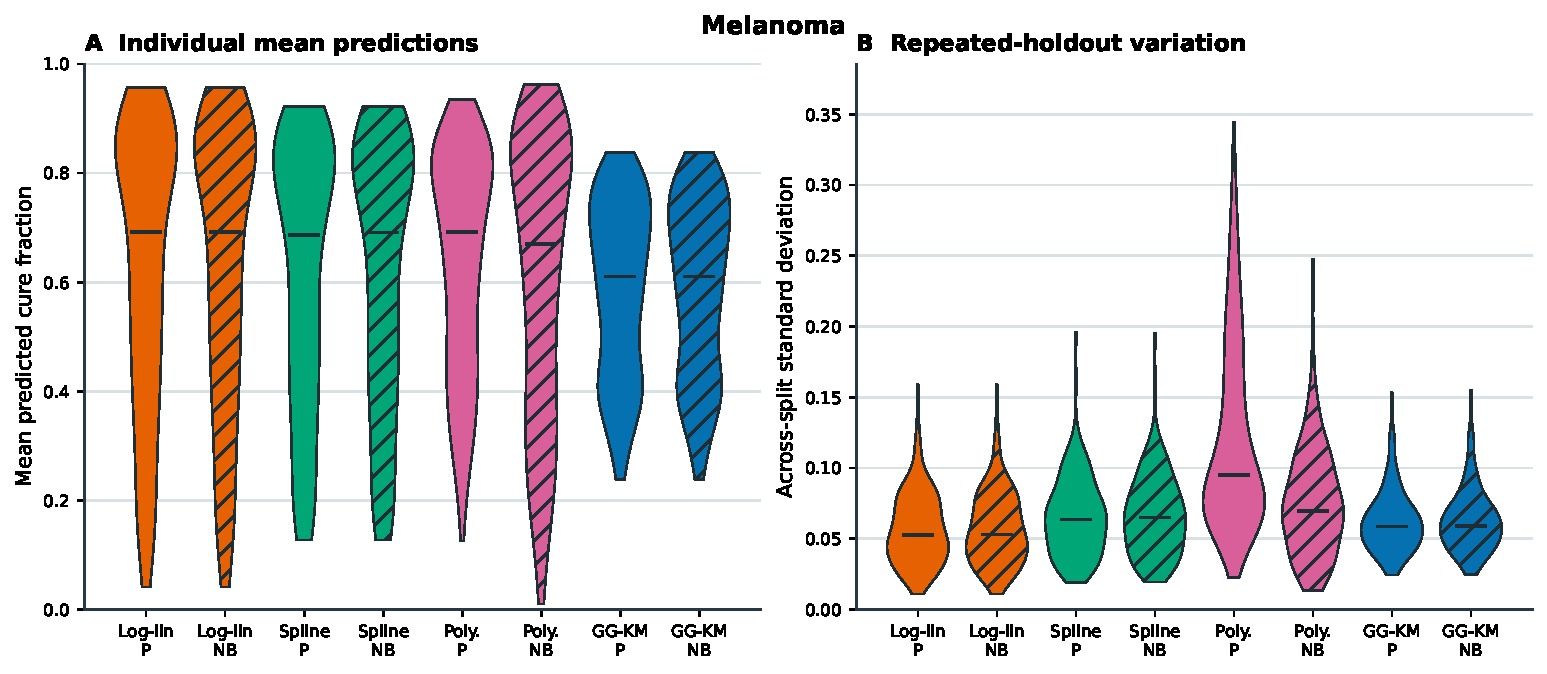
\includegraphics[width=\textwidth]{melanoma_individual_cure_variation.pdf}
\caption{Descriptive individual cure-fraction predictions in the melanoma repeated-holdout analysis. Panel A shows the distribution across patients of each individual's mean out-of-sample prediction. Panel B shows the distribution of within-individual standard deviations across outer test-set appearances. P denotes Poisson and NB denotes negative binomial; hatched distributions correspond to negative-binomial models.}
\label{fig:supp-melanoma-cure}
\end{figure}

\begin{figure}[tbp]
\centering
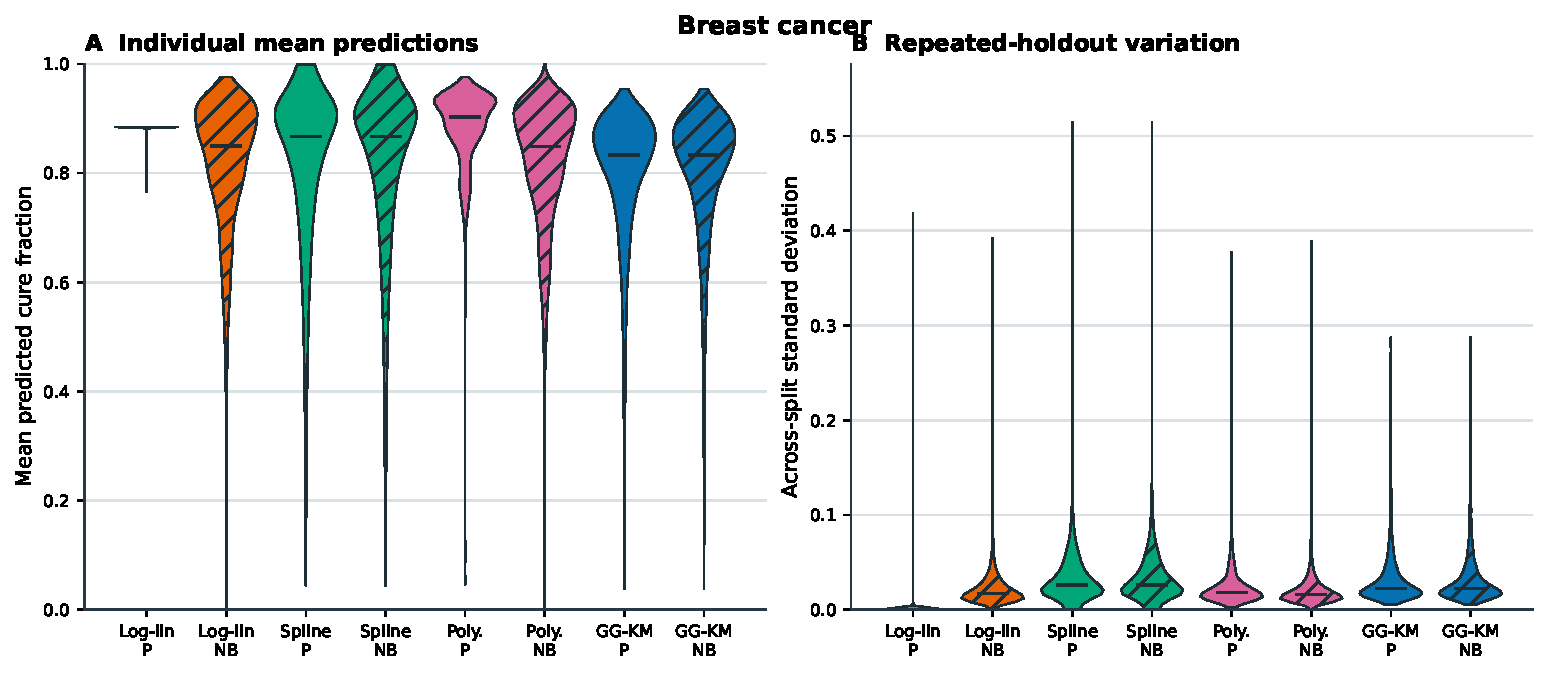
\includegraphics[width=\textwidth]{breast_cancer_individual_cure_variation.pdf}
\caption{Descriptive individual cure-fraction predictions in the breast cancer repeated-holdout analysis. Panel A shows the distribution across patients of each individual's mean out-of-sample prediction. Panel B shows the distribution of within-individual standard deviations across outer test-set appearances. P denotes Poisson and NB denotes negative binomial; hatched distributions correspond to negative-binomial models.}
\label{fig:supp-breast-cancer-cure}
\end{figure}


\section{Reproducibility record}\label{sec:supp-reproducibility}

The scripts for reproducing the simulation, melanoma, and breast cancer analyses and generating their figures and tables are available at \url{https://github.com/cowvin0/ggkm_paper}.

To reproduce all simulation, melanoma, and breast cancer results, activate a Python environment with the required dependencies and make the original clinical datasets available in the project's \path{data/} directory. Run the following command from the project root on a PBS cluster:
\begin{verbatim}
python scripts/run_workflow.py --mode cluster
\end{verbatim}
The workflow submits the experiment jobs and generates each dataset's figures and tables after its experiment array finishes successfully.

To run the same complete workflow on a local machine, use:
\begin{verbatim}
python scripts/run_workflow.py --mode local
\end{verbatim}

The analyses use deterministic random seeds and one numerical thread per worker.

If the experiment results are already available, regenerate only the figures and tables with:
\begin{verbatim}
python scripts/run_workflow.py --mode cluster --stage postprocess
\end{verbatim}
Replace \texttt{cluster} with \texttt{local} to regenerate them locally. The saved CSV and NPZ results and the original clinical datasets must be available on the machine performing this step. Figures are saved in \path{figures/review/}, and tables in \path{sections/generated/}.

The experiment routines save CSV results and compressed NPZ prediction and diagnostic archives used to regenerate the figures and tables. Workflow execution records are saved by default in \path{logs/workflow/}, and cluster job logs in \path{logs/pbs/}.
\end{document}
